\documentclass{article}

\usepackage[letterpaper,margin=1in,footskip=0.25in]{geometry}
\usepackage[nottoc,notlof,notlot,numbib]{tocbibind}
\usepackage{fancyhdr}
\usepackage{graphicx}
\usepackage{amsmath}
\usepackage{subcaption}
\usepackage[hidelinks]{hyperref}
\usepackage{csquotes}

\MakeOuterQuote{"}

\title{The Christmas Tree Problem}
\author{Steven Labalme}
\date{\today}

\begin{document}




\pagenumbering{gobble}
\maketitle
\newpage



\pagenumbering{roman}
\tableofcontents
\listoffigures
\newpage



\pagenumbering{arabic}
\pagestyle{fancy}
\fancyhf{}
\rfoot{Labalme \thepage}
\renewcommand{\headrulewidth}{0em}
\setcounter{secnumdepth}{0}
\begin{center}
\section{Abstract}
\end{center}

\begin{figure}[h!]
    \centering
    \begin{subfigure}{0.3\linewidth}
        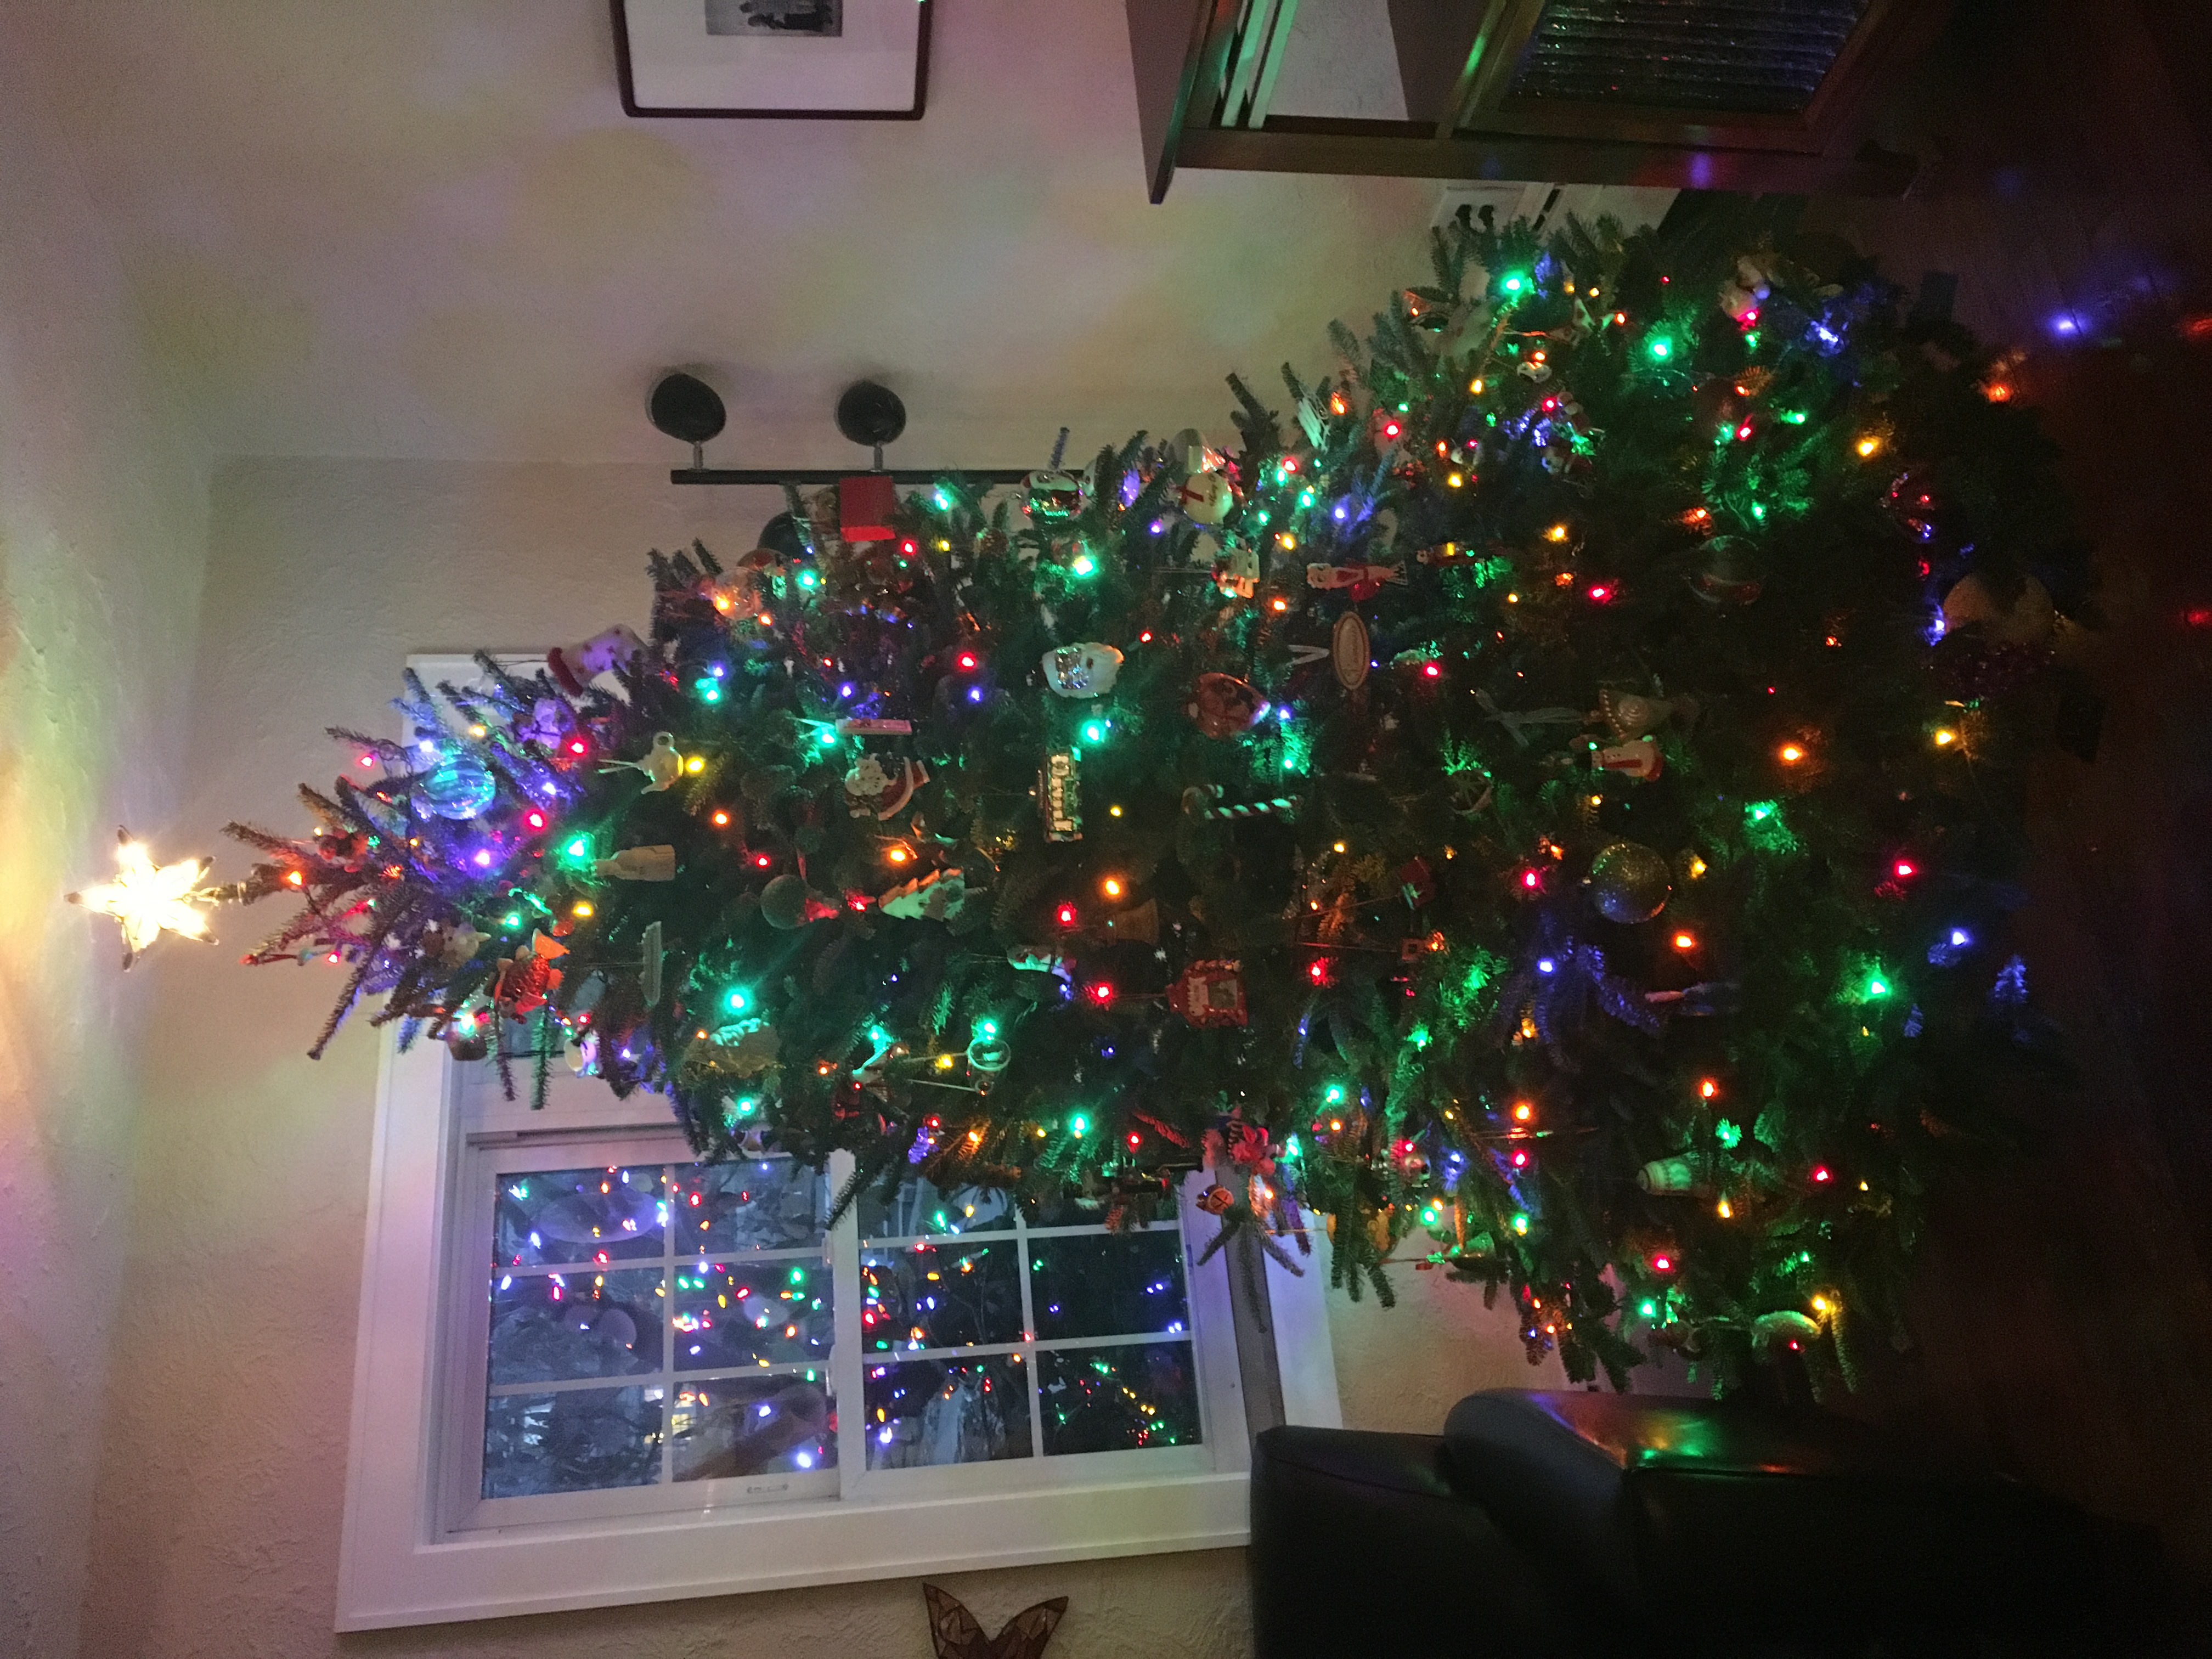
\includegraphics[width=\linewidth]{Blender/christmastree.png}
        \caption{A Christmas tree.}
        \label{fig:helixa}
    \end{subfigure}
    \begin{subfigure}{0.4\linewidth}
        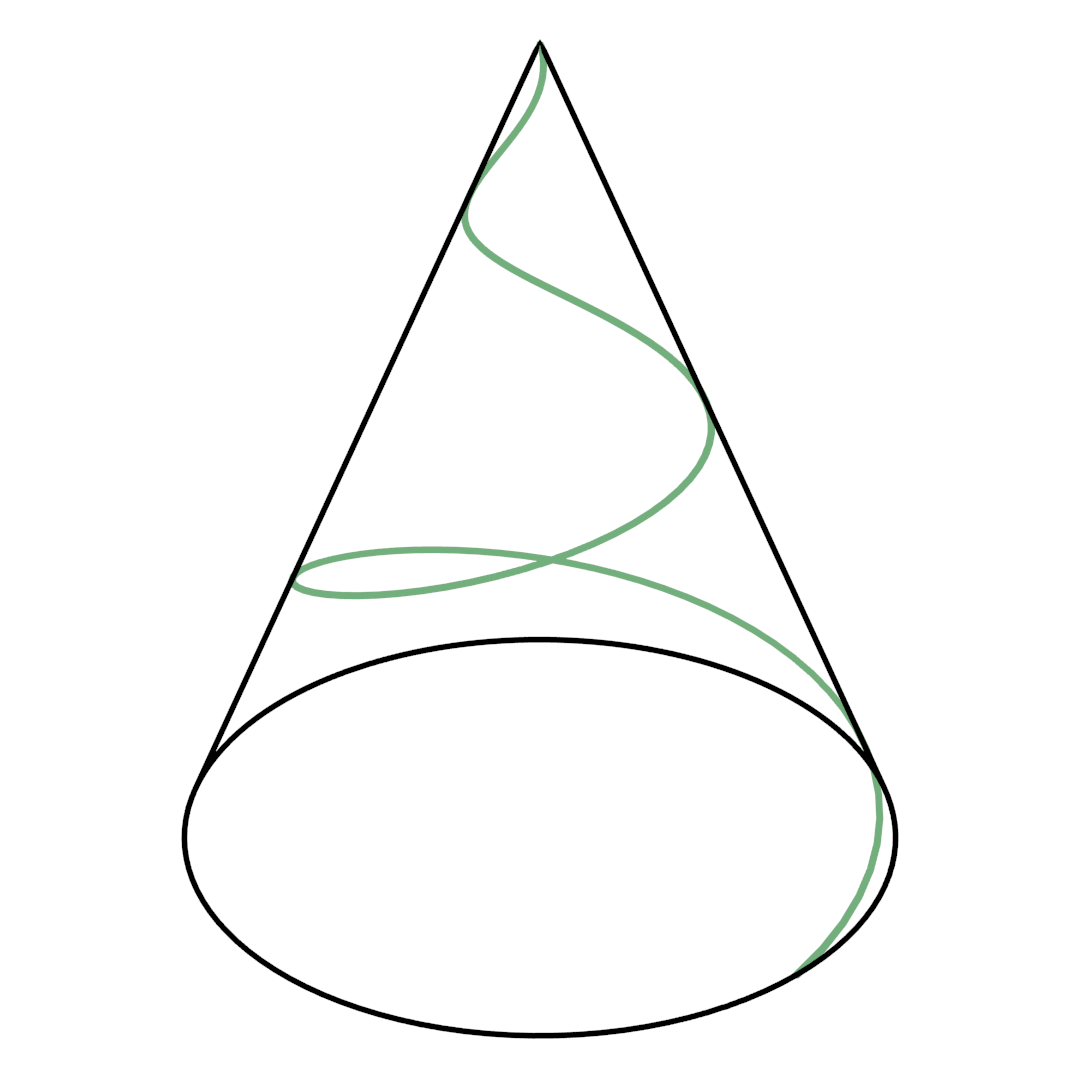
\includegraphics[width=\linewidth]{Blender/helix.png}
        \caption{A conical helix and its cone.}
        \label{fig:helixb}
    \end{subfigure}
    \caption{Simplification of Christmas tree lights/tinsel.}
    \label{fig:helix}
\end{figure}

Around December 25 every year, millions of families around the world cut down a small evergreen tree to bring into their homes and adorn with ornaments, lights, and sometimes tinsel. An annual conundrum for such families is trying to determine how many strands of lights are necessary. By idealizing a Christmas tree, such as the one pictured in Figure \ref{fig:helixa}, to a cone, such as is seen in Figure \ref{fig:helixb}, and the lights to a one-dimensional strand wrapped around the "tree" in perfectly spaced intervals, the length of such a "strand of lights" can be found using integral calculus.\par
Oftentimes, three-dimensional mathematics is the realm of planes and surfaces --- the output of an equation in the form, $z(x,y)$. However, this paper is understandably concerned with three-dimensional lines, specifically those technically defined as conical helices$^[$\footnote{A spiral on the surface of a cone of revolution.}$^]$. In addition to volume, arc length is commonly taught at the AP BC Calculus level as an application of integral calculus. This paper derives two expressions for the conical helix spun $n$ times around a cone of base radius, $r$, and height, $h$ and two three-dimensional arc length function. These are then deployed to find a general formula for the length of such a helix.\par
The conclusion of each section was identical. Every method supports the hypothesis that the length, $\ell$, of this class of conical helices as a function of $n$, $h$, and $r$ is given by
\begin{equation*}
    \ell = \sqrt{(\pi nr)^2+\frac{1}{4}\left(r^2+h^2\right)}-\frac{r^2+h^2}{4\pi nr}\ln\Bigg|\frac{\sqrt{(2\pi nr)^2+r^2+h^2}-2\pi nr}{\sqrt{r^2+h^2}}\Bigg|
\end{equation*}
\newpage



\setcounter{secnumdepth}{3}
\section{Multivariable Parametric Equations}
\subsection{Introduction}

\begin{figure}[h!]
    \centering
    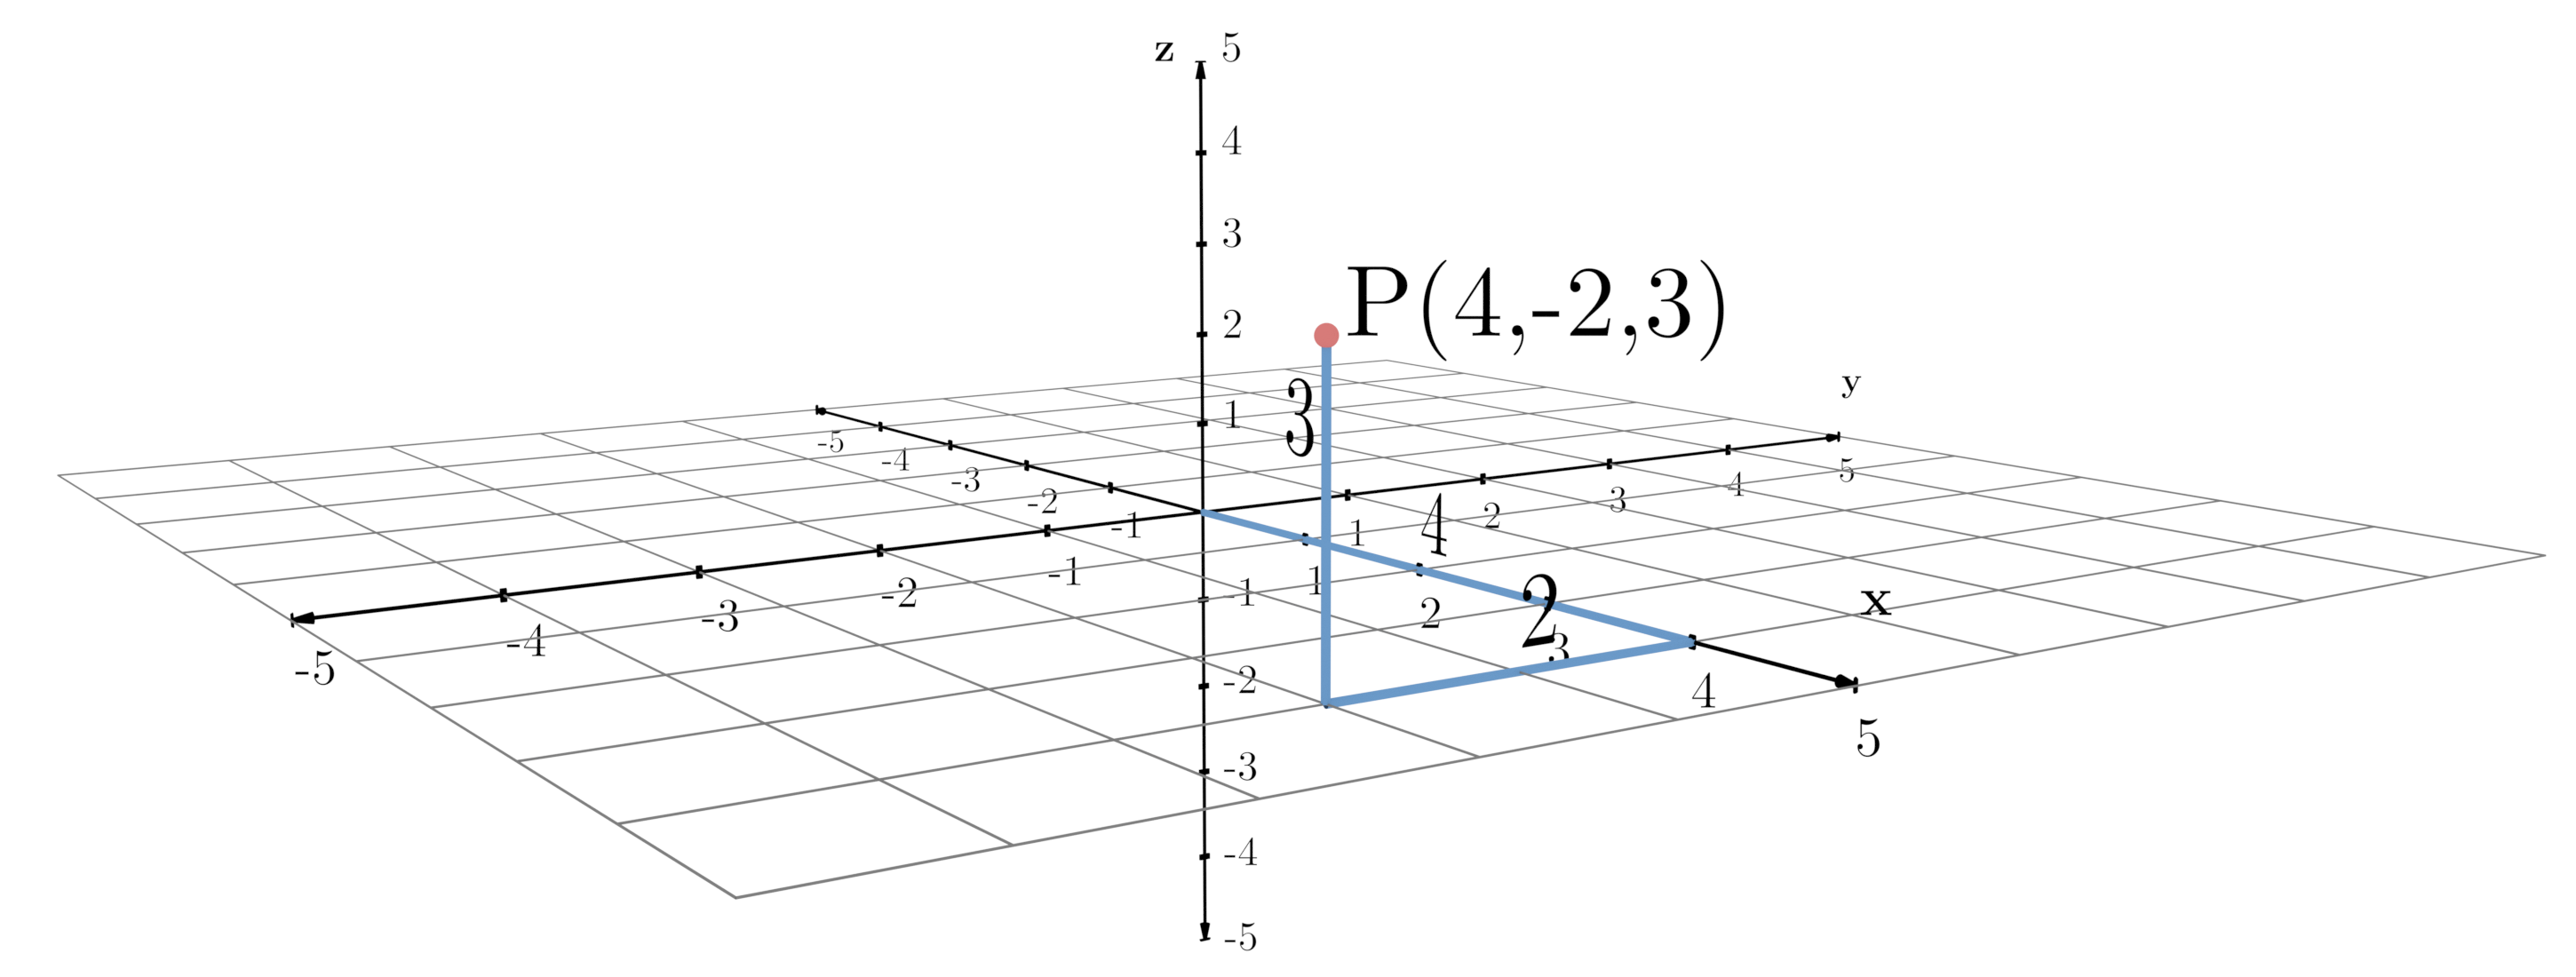
\includegraphics[width=0.711\linewidth]{Blender/cartesian.png}
    \caption{3D Cartesian coordinate system.}
    \label{fig:cart}
\end{figure}

According to Harrison, it is possible to describe curves in three dimensions using parameterizations. These curves can vary widely, but this paper will focus on conical helices (see Figure \ref{fig:helixb}; Harrison parameterizes one example of such a curve). The method that he employs makes use of the Cartesian coordinate system$^[$\footnote{This defines a point using three numbers, each of which corresponds to the magnitude of a vector pointing away from the origin. The point is at the sum of these vectors. The dot product of any two of these vectors is zero.}$^]$ (Figure \ref{fig:cart}). Lastly, it is possible to find the arc length using integral calculus and the 3D arc length formula \cite{Bib:param}.\par
First, it is necessary to determine the parameterization for the general conical helix. The simpler, related cylindrical helices will be used as the foundation for this derivation. Next, it is necessary to derive the 3D distance formula, which is instrumental in the subsequent derivation of the 3D arc length formula. Lastly, the parameterization is plugged into the arc length formula and simplified.


\subsection{Derivation}
\paragraph{THEOREM} The length of the helix spun $n$ times around the surface of a cone of base radius, $r$, and height, $h$, is $\sqrt{(\pi nr)^2+\frac{1}{4}\left(r^2+h^2\right)}-\frac{r^2+h^2}{4\pi nr}\ln\bigg|\frac{\sqrt{(2\pi nr)^2+r^2+h^2}-2\pi nr}{\sqrt{r^2+h^2}}\bigg|$ where $n,\ r,\ h>0$.

\begin{figure}[h!]
    \centering
    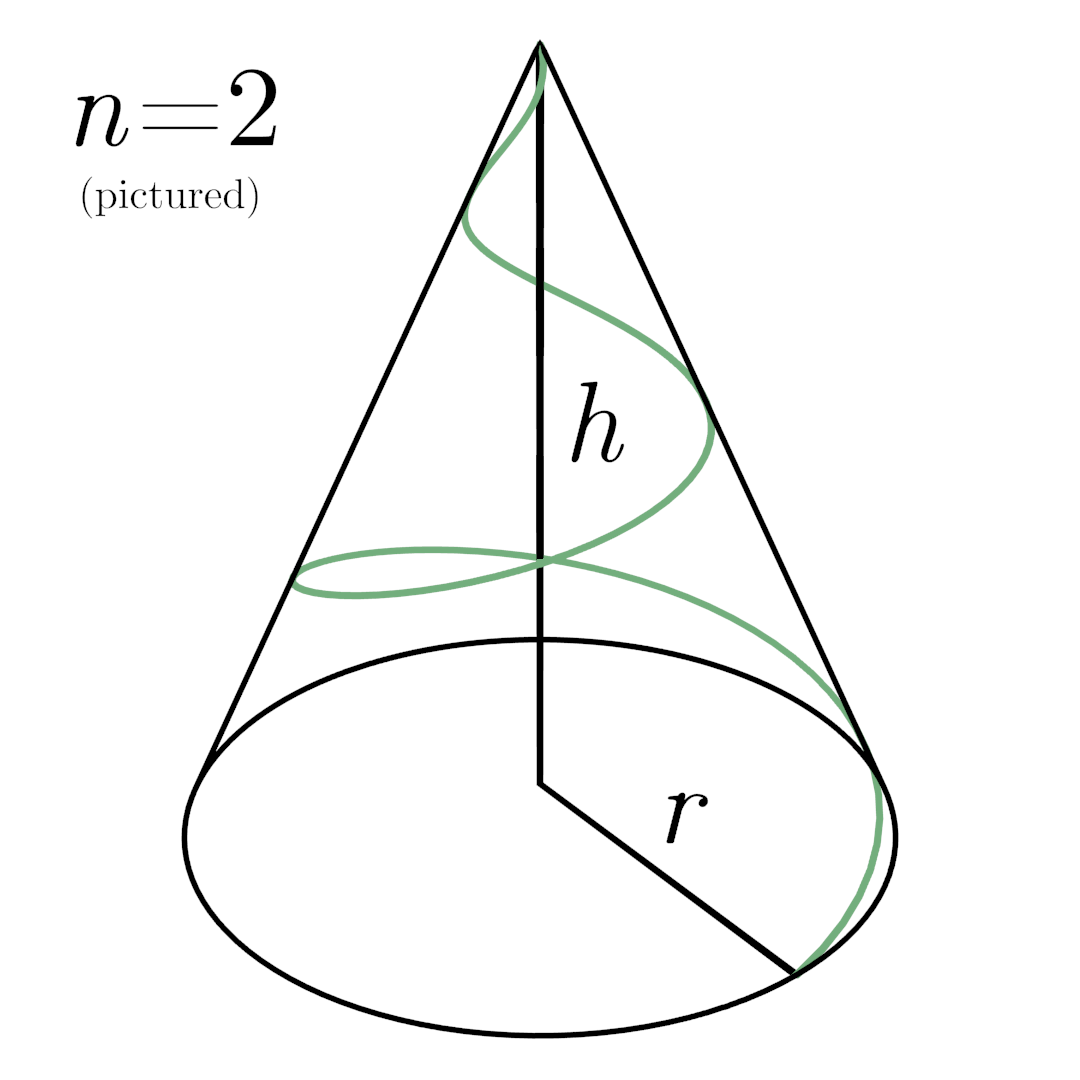
\includegraphics[width=0.4\linewidth]{Blender/helixlab.png}
    \caption{A variable conical helix and cone.}
    \label{fig:helixlab}
\end{figure}

\paragraph{PROOF} Begin by deriving a parameterization of the conical helix both defined by the theorem above and of the type shown in Figure \ref{fig:helixlab}. Since the cone is a three-dimensional figure, this will not be a parameterization in $x$ and $y$ but a parameterization in $x$, $y$, and $z$. However, 2D curves can be helpful in deriving the three equations for this helix. Instead of immediately trying to derive the equations for a conical helix, start by deriving equations for a cylindrical helix.

\begin{figure}[h!]
    \centering
    \begin{subfigure}{0.3\linewidth}
        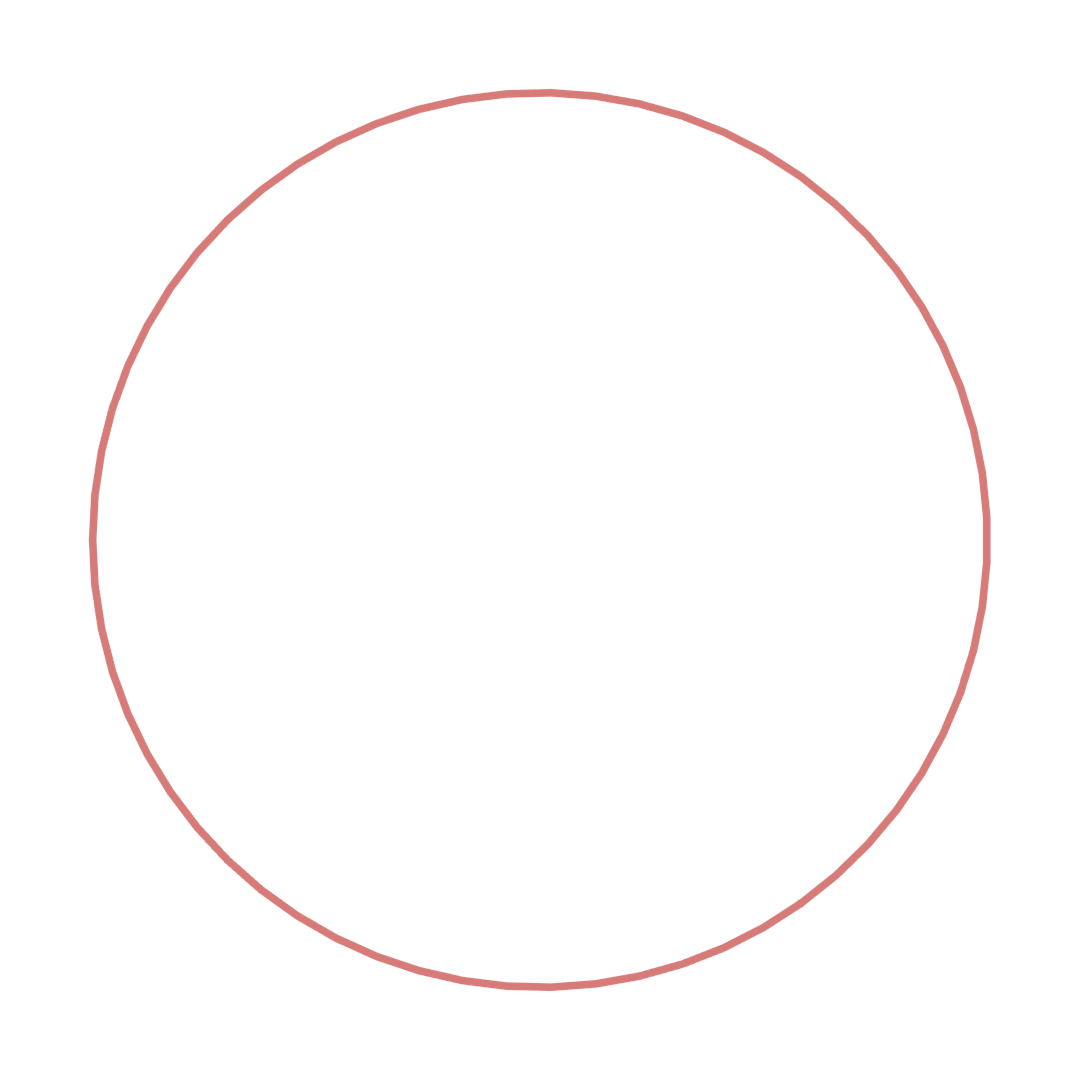
\includegraphics[width=\linewidth]{Blender/helixca.png}
        \caption{Parameterized circle.}
        \label{fig:helixca}
    \end{subfigure}
    \begin{subfigure}{0.3\linewidth}
        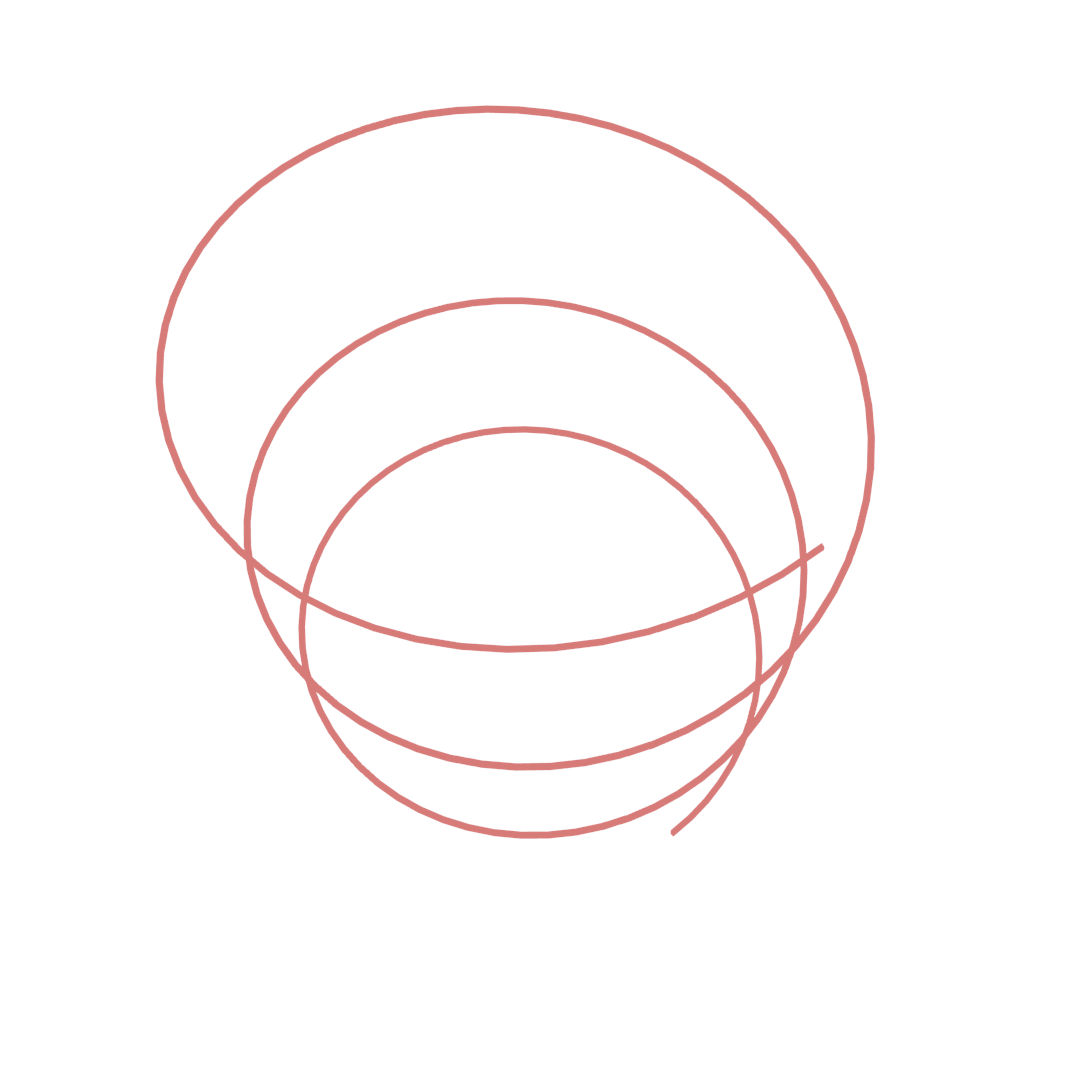
\includegraphics[width=\linewidth]{Blender/helixcb.png}
        \caption{Cylindrical helix.}
        \label{fig:helixcb}
    \end{subfigure}
    \begin{subfigure}{0.3\linewidth}
        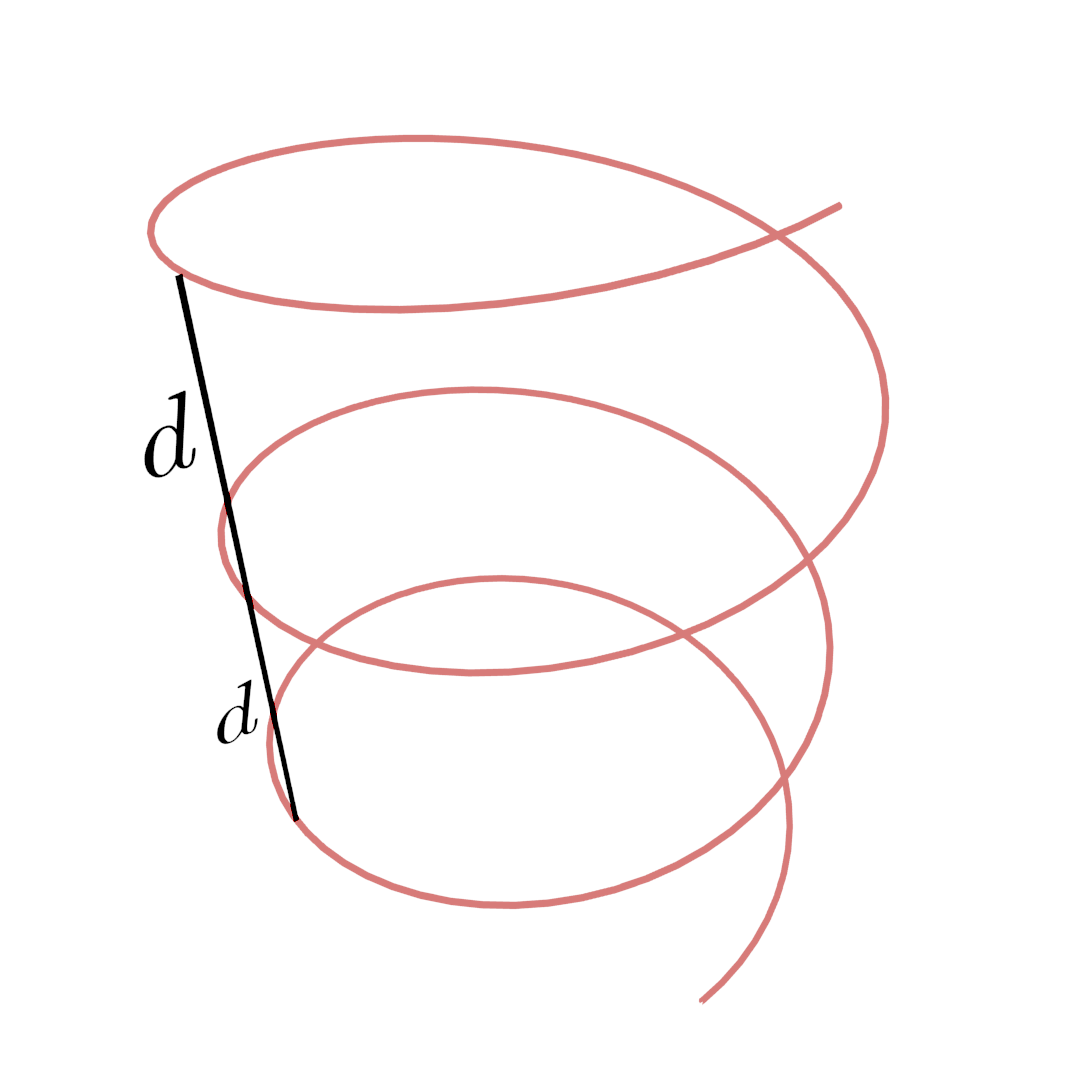
\includegraphics[width=\linewidth]{Blender/helixcc.png}
        \caption{Helix with adjacent points.}
        \label{fig:helixcc}
    \end{subfigure}
    \caption{Circle $\longrightarrow$ cylindrical helix.}
    \label{fig:helixc}
\end{figure}

Let's start with the two-dimensional equivalent of a cylindrical helix --- a circle$^[$\footnote{A cylindrical helix viewed from above is a circle, as shown by the left-right progression in Figure \ref{fig:helixc}.}$^]$. To draw a circle of radius $r$, it is possible to use the parameterization,
\begin{align*}
    x(t) &= r\cos(2\pi t)\\
    y(t) &= r\sin(2\pi t)
\end{align*}
where $t\in[0,1]$. What these equations reveal is that the sine and cosine functions can draw a circle$^[$\footnote{This does make sense because both sine and cosine are intrinsically related to triangles within the unit circle.}$^]$.\par
Now, it is necessary to extend the circle into three dimensions, as seen in Figure \ref{fig:helixcb}. One important characteristic of a cylindrical helix is that there is a constant distance between adjacent points, as seen in Figure \ref{fig:helixcc} ($d=d$). What this means is that the height, $z$, of each point is increasing constantly (as opposed to parabolically, logarithmically, or some other variable rate of growth).\par
The equation for constant growth in the $z$-direction is therefore $z=c_1t+c_2$, where $c_1$ and $c_2$ are constants. An equation in this form will always be a straight line (have a constant rate of growth). If this equation is added, the complete parameterization for a cylindrical helix of radius, $r$, height per spiral, $c_1$, and height offset, $c_2$, is revealed, as follows.
\begin{align}\label{eqns:helixc}
    \begin{split}
        x(t) &= r\cos(2\pi t)\\
        y(t) &= r\sin(2\pi t)\\
        z(t) &= c_1t+c_2
    \end{split}
\end{align}
Note that the number of spirals is controlled by the domain of $t$, i.e. if $t$ varies from $0$ to $3$, there will be $3$ spirals, all of which are above the $xy$-plane. Now that the parameterization for a cylindrical helix has been obtained (equations \ref{eqns:helixc}), it is possible to modify them to determine the one for the conical helix in Figure \ref{fig:helixlab}.\par
Before tackling the conical shape (a variation of the radius, $r$, over the range of heights), begin by inserting the variables $h$ and $n$. The variable, $h$, is the height of the cone. However, to define height requires defining a start and end point for $t$ (otherwise the helix would be infinite). Because different values of $c_1$ and $c_2$ in equations \ref{eqns:helixc} can modify any range of $t$ to equal any other, the range of $t$ is arbitrary, so choose the simple,
\begin{equation}\label{eqn:int}
    t\in[0,1]
\end{equation}
As to $c_2$, arc length does not depend on the $z$-position of the helix, so choose $c_2=0$ to simplify matters. For $c_1$, consider that the first point of the helix (when $t=0$) should correspond to height, $0$, while the last point of the helix (when $t=1$) should correspond to height, $h$. As such, employ the slope formula and simplify.
\begin{align*}
    c_2 &= \frac{\Delta z}{\Delta t}\\
    &= \frac{h-0}{1-0}\\
    &= h
\end{align*}
Therefore, the $z$-parameterization for the conical helix should be
\begin{equation}\label{eqn:z}
    z(t)=ht
\end{equation}\par
The variable, $n$, is the number of revolutions the helix completes around the cone. With the parameterization given by equations \ref{eqns:helixc}, the helix spirals once over the chosen range of $t$. Properties of sinusoids can reveal that if the coefficients of $t$ in the $x(t)$ and $y(t)$ equations were doubled, two revolutions would be completed. If they were tripled, three revolutions would be completed. This direct correlation allows the following modification to insert $n$.
\begin{align}\label{eqns:xy}
    \begin{split}
        x(t) &= r\cos(2\pi nt)\\
        y(t) &= r\sin(2\pi nt)
    \end{split}
\end{align}
Now for the variable, $r$. Regard Figure \ref{fig:coneside}, which shows the helix from an orthographic side view and a line connecting the first and last points of the helix. This line is representative of the radius-height relationship, for at every height, $z(t)$, the radius of the helix is the distance between the line and the $z$-axis. This is key --- because a cone's side-view projection is a triangle, the radius of a conical helix varies \emph{linearly} with height.

\begin{figure}[h!]
    \centering
    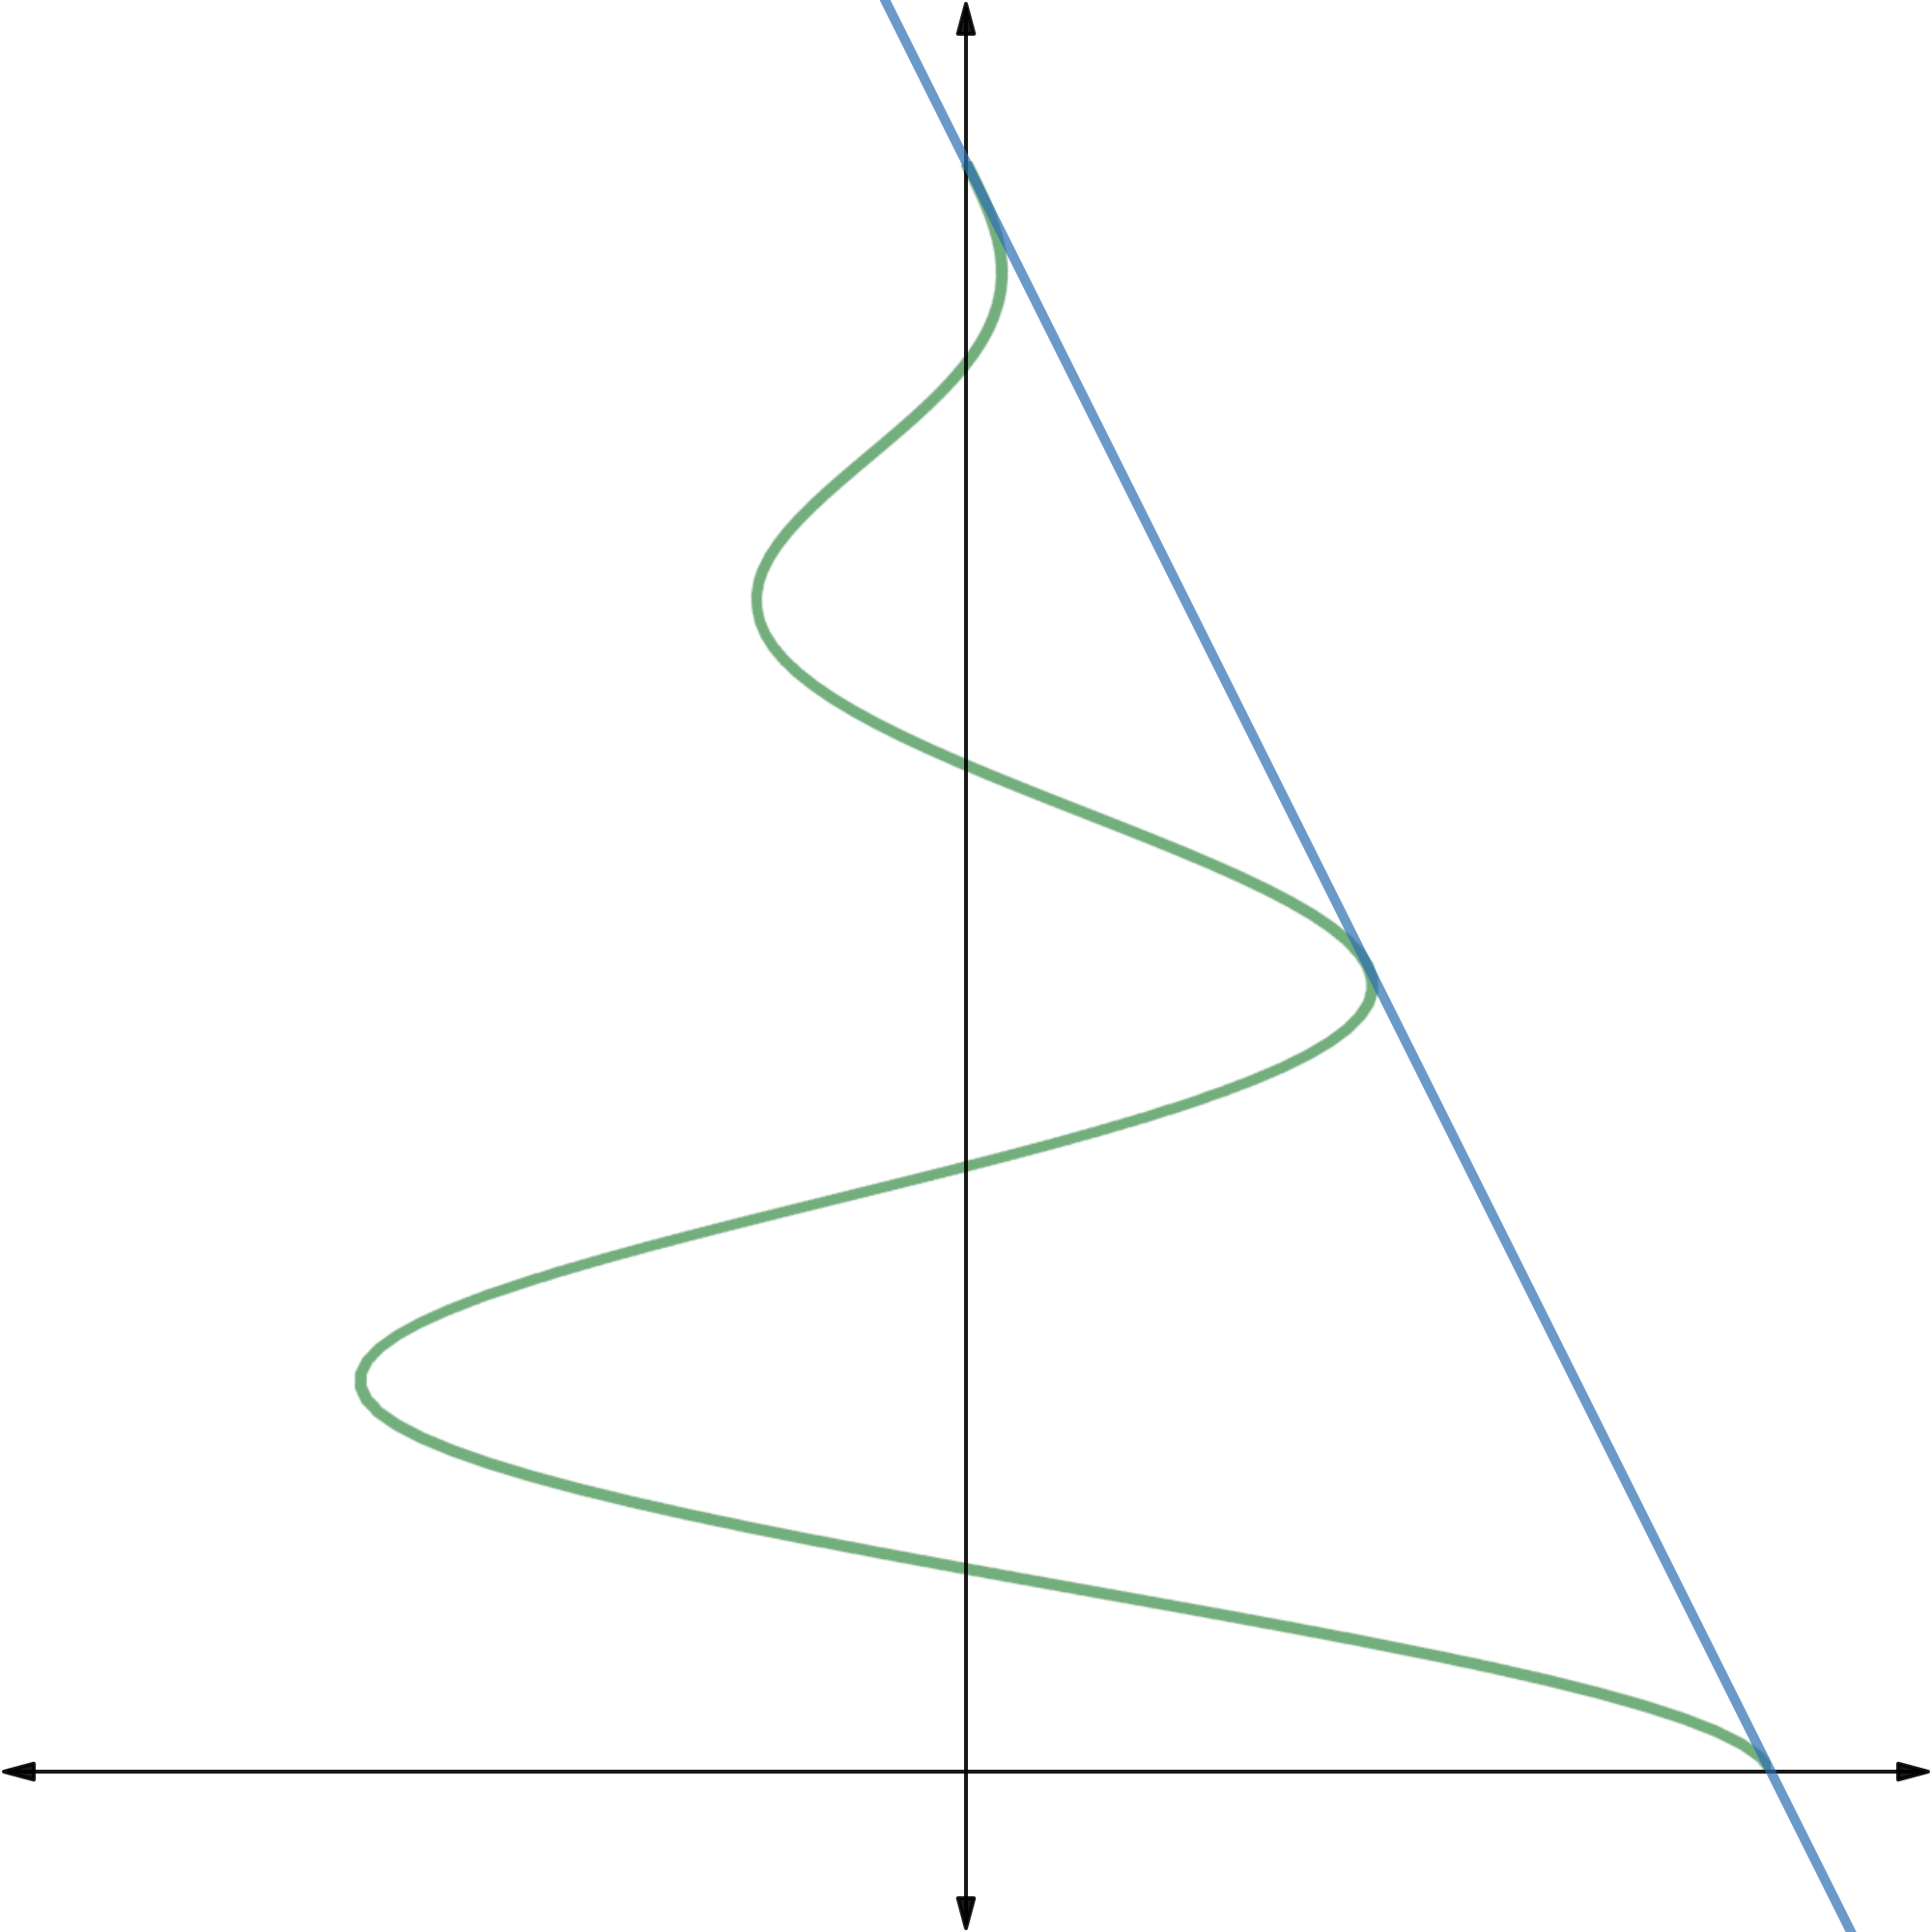
\includegraphics[width=0.4\linewidth]{Blender/ConeSide-f.png}
    \caption{Radius of the conical helix.}
    \label{fig:coneside}
\end{figure}

To change the radius of the conical helix, modify the $x(t)$ and $y(t)$ equations with the goal of changing the amplitude$^[$\footnote{A measure of the change in a periodic variable over a single period. In layman's terms, the distance between the highest and lowest point of a sinusoid in one wave.}$^]$ of the sinusoids. The amplitude at $t=0$ must be $r$, while the amplitude at $t=1$ must be $0$, and there is a linear relationship between $h$ and $r$. Because $h$ and $t$ are linearly related, there is a linear relationship between $t$ and $r$. Therefore, employ point-slope form along with the slope formula and simplify as follows to yield the equation for the radius/amplitude, $r(t)$.
\begin{align*}
    r(t)-r &= \frac{\Delta r}{\Delta t}(t-0)\\
    r(t) &= r+\frac{0-r}{1-0}t\\
    r(t) &= r-rt\tag{\theequation}\label{eqn:rt}
    \stepcounter{equation}
\end{align*}
Replace the current amplitude, $r$, in $x(t)$ and $y(t)$ of equations \ref{eqns:xy} with the right side of equation \ref{eqn:rt} and substitute equation \ref{eqn:z} for $z(t)$ to yield the final parameterization of the conical helix (equations \ref{eqns:helixcn}). The reader can use a 3D helix simulation, such as Christopher Chudzicki's \cite{Bib:sim}, to interact with these equations with variables of their choice$^[$\footnote{Make sure to write the equations in Python code, e.g. it is \textit{always} necessary to use an asterisk to signify multiplication.}$^]$.
\begin{align}\label{eqns:helixcn}
    \begin{split}
        x(t) &= (r-rt)\cos(2\pi nt)\\
        y(t) &= (r-rt)\sin(2\pi nt)\\
        z(t) &= ht
    \end{split}
\end{align}

\bigskip
Now that the parameterization has been obtained, the length of the defined helix can be found. However, the general three-dimensional arc length formula will be derived first. If the two-dimensional arc length formula was derived from the 2D distance formula, a logical place to start now would be the 3D distance formula. This will also be briefly derived.

\begin{figure}[h!]
    \centering
    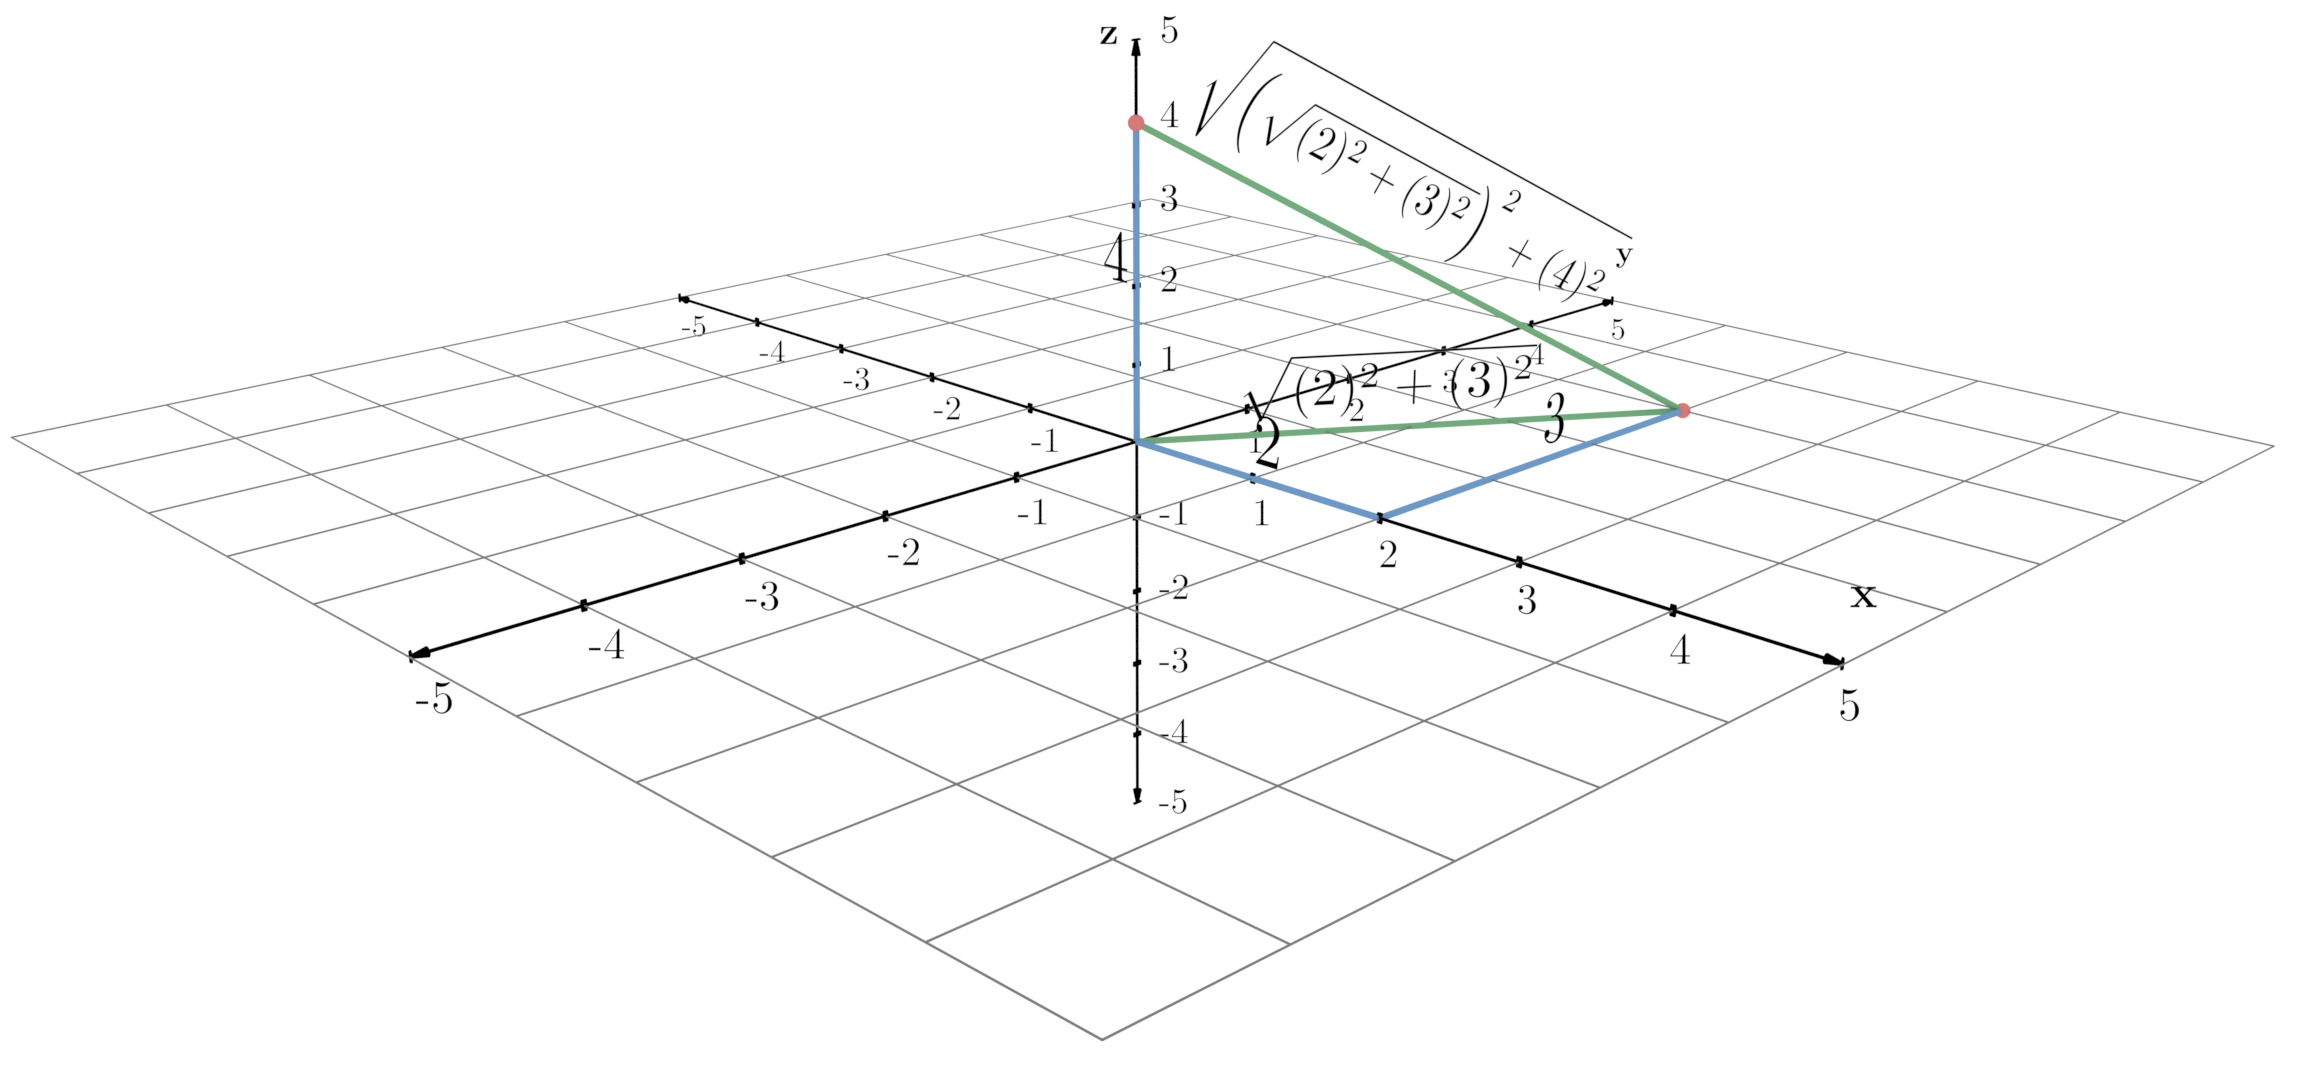
\includegraphics[width=0.711\linewidth]{Blender/3Ddist.png}
    \caption{3D distance formula.}
    \label{fig:3Ddist}
\end{figure}

Regard Figure \ref{fig:3Ddist}. The Pythagorean Theorem generates the 2D distance formula with $\Delta x$ and $\Delta y$ as the inputs. In 3D, use the 2D distance formula once with $\Delta x$ and $\Delta y$ and then again with the new arm and $\Delta z$. Then simplify. Mathematically,
\begin{align*}
    \sqrt{(\Delta x)^2+(\Delta y)^2} &\rightarrow \sqrt{\left(\sqrt{(\Delta x)^2+(\Delta y)^2}\right)^2+(\Delta z)^2}\\
    &= \sqrt{(\Delta x)^2+(\Delta y)^2+(\Delta z)^2}\tag{\theequation}\label{eqn:3Ddist}
    \stepcounter{equation}
\end{align*}\par
Now it's possible to derive the 3D arc length formula. This process has very similar steps to the 2D version, explained by Paul Dawkins \cite{Bib:2Darc}. First, notice that it is not possible to directly find the length of the helix using regular geometric formulas$^[$\footnote{Examples include $2\pi r$ for the perimeter of a circle and $ns$ for the perimeter of an $n$-gon.}$^]$. However, it can be approximated using multiple line segments, the length of which can be found using equation \ref{eqn:3Ddist}. As more and more, smaller and smaller segments are used, the estimated length will approach the actual length. This limit can be found using integration$^[$\footnote{Integration sums infinitely many infinitely small pieces.}$^]$.\par

\begin{figure}[h!]
    \centering
    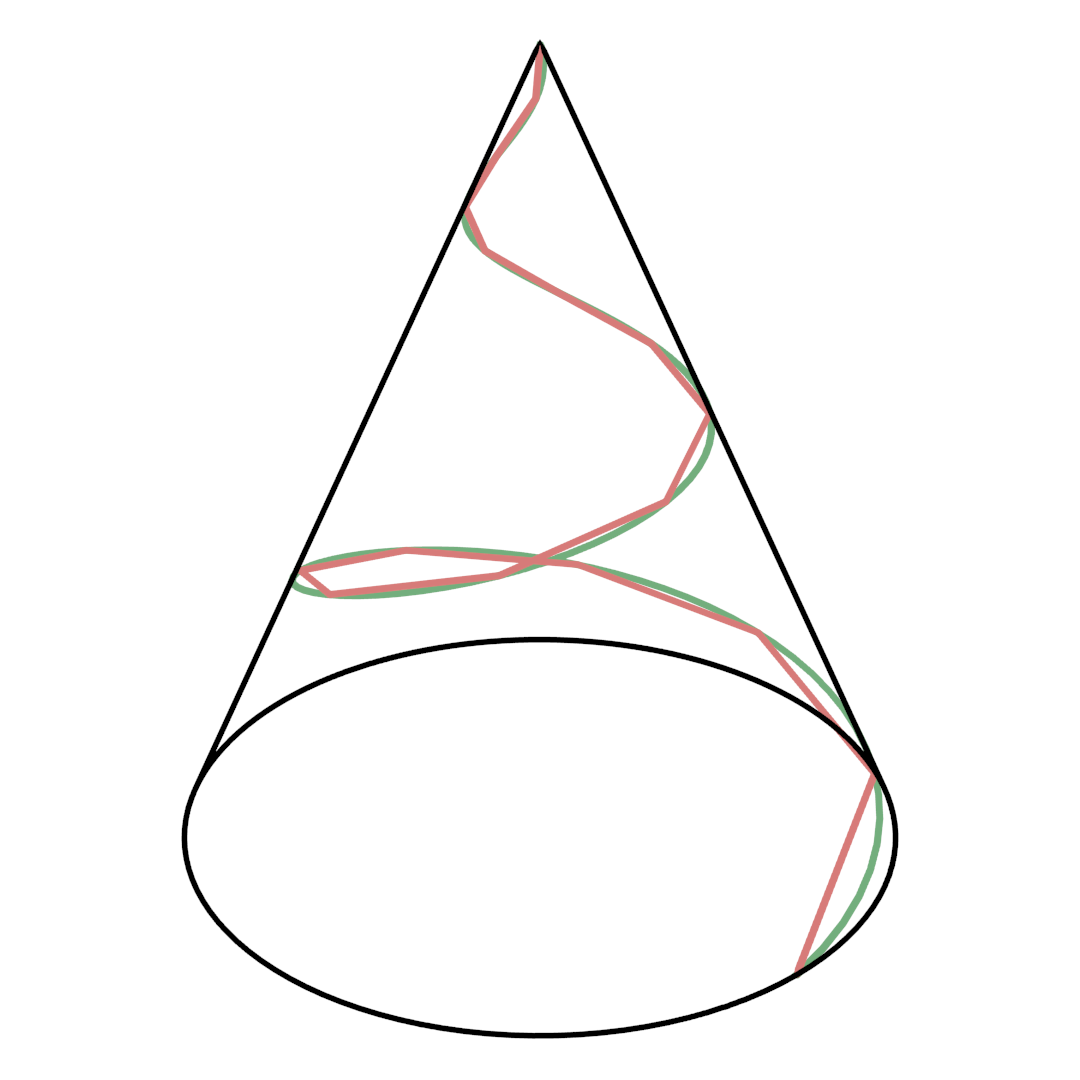
\includegraphics[width=0.4\linewidth]{Blender/helixsegs.png}
    \caption{The conical helix as approximated by line segments.}
    \label{fig:helixsegs}
\end{figure}

Take the conical helix of Figure \ref{fig:helixlab} and imagine transforming it into a connection of line segments, as shown in Figure \ref{fig:helixsegs}.\par
Each line segment, by definition, has both endpoints on the helix. For example, if the coordinates of one point are given by $f(t)$ (where $f(t)$ is defined by equations \ref{eqns:helixcn}) for some value of $t$ on interval \ref{eqn:int} then the coordinates of the next point would be given by $f(t+\Delta t)$. The length of this arbitrary line segment can be found using equation \ref{eqn:3Ddist}, as follows. Note that each "Delta variable" is exchanged for the final condition minus the initial condition and that $d$ is used to signify the distance between two endpoints of a segment.
\begin{equation*}
    d = \sqrt{(x(t+\Delta t)-x(t))^2+(y(t+\Delta t)-y(t))^2+(z(t+\Delta t)-z(t))^2}
\end{equation*}
Multiply the above equation by a form of $1$, namely $\frac{\Delta t}{\Delta t}$.
\begin{equation*}
    d = \sqrt{(x(t+\Delta t)-x(t))^2+(y(t+\Delta t)-y(t))^2+(z(t+\Delta t)-z(t))^2}\times\frac{\Delta t}{\Delta t}
\end{equation*}
Rewrite a few times to maneuver the denominator under the radical and distribute it to each term.
\begin{align*}
    d &= \frac{1}{\Delta t}\sqrt{(x(t+\Delta t)-x(t))^2+(y(t+\Delta t)-y(t))^2+(z(t+\Delta t)-z(t))^2}\ \Delta t\\
    &= \sqrt{\frac{1}{(\Delta t)^2}}\sqrt{(x(t+\Delta t)-x(t))^2+(y(t+\Delta t)-y(t))^2+(z(t+\Delta t)-z(t))^2}\ \Delta t\\
    &= \sqrt{\frac{(x(t+\Delta t)-x(t))^2+(y(t+\Delta t)-y(t))^2+(z(t+\Delta t)-z(t))^2}{(\Delta t)^2}}\ \Delta t\\
    &= \sqrt{\frac{(x(t+\Delta t)-x(t))^2}{(\Delta t)^2}+\frac{(y(t+\Delta t)-y(t))^2}{(\Delta t)^2}+\frac{(z(t+\Delta t)-z(t))^2}{(\Delta t)^2}}\ \Delta t\\
    &= \sqrt{\left(\frac{x(t+\Delta t)-x(t)}{\Delta t}\right)^2+\left(\frac{y(t+\Delta t)-y(t)}{\Delta t}\right)^2+\left(\frac{z(t+\Delta t)-z(t)}{\Delta t}\right)^2}\ \Delta t\tag{\theequation}\label{eqn:length}
    \stepcounter{equation}
\end{align*}
The outputs of equation \ref{eqn:length} above can be summed as $t$ varies along the interval. As $\Delta t$ grows smaller and more iterations are summed, the estimate given by the sums of equation \ref{eqn:length} becomes more accurate. These rewrites to obtain equation \ref{eqn:length} may seem unnecessary until the reader remembers the task at hand: to integrate.\par
They have accomplished two major tasks. First, they have put a $\Delta t$ as a coefficient to the body of the equation. This piece is necessary because integration transforms this term into $dt$, the variable of integration. Second, each of the three terms under the radical looks suspiciously like the square of the limit definition of the derivative. Indeed, as integration minimizes the $\Delta t$ at the end of the equation to infinitesimal proportions, it will transform each expression into the derivative of its respective variable. Therefore, rewrite equation \ref{eqn:length} above as an integrable statement. Note that $\ell$ is used to signify the length of the helix.
\begin{equation}\label{eqn:arcparam}
    \ell = \int_a^b\sqrt{\left(\frac{dx}{dt}\right)^2+\left(\frac{dy}{dt}\right)^2+\left(\frac{dz}{dt}\right)^2}\, dt
\end{equation}
Equation \ref{eqn:arcparam} above is the 3D arc length formula for an $xyz$-parameterized curve, such as equations \ref{eqns:helixcn}.

\bigskip
Plug equations \ref{eqns:helixcn} into equation \ref{eqn:arcparam} and evaluate. Use the bounds given by interval \ref{eqn:int}.
\begin{align*}
    \ell &= \int_0^1\sqrt{\left(\frac{d}{dt}((r-rt)\cos(2\pi nt))\right)^2+\left(\frac{d}{dt}((r-rt)\sin(2\pi nt))\right)^2+\left(\frac{d}{dt}(ht)\right)^2}\, dt\\
    &= \int_0^1\sqrt{(-r\cos(2\pi nt)-2\pi n(r-rt)\sin(2\pi nt))^2+(-r\sin(2\pi nt)+2\pi n(r-rt)\cos(2\pi nt))^2+(h)^2}\, dt\\
    &= \int_0^1\sqrt{(2\pi n(r-rt)\sin(2\pi nt)+r\cos(2\pi nt))^2+(2\pi n(r-rt)\cos(2\pi nt)-r\sin(2\pi nt))^2+h^2}\, dt
\end{align*}
For the sake of simplicity, use the following substitutions.
\begin{align*}
    u &= 2\pi n(r-rt)&
    v &= 2\pi nt
\end{align*}
Continue the evaluation.
\begin{align*}
    \ell &= \int_{t=0}^1\sqrt{(u\sin(v)+r\cos(v))^2+(u\cos(v)-r\sin(v))^2+h^2}\, dt\\
    &= \int_{t=0}^1\sqrt{u^2\sin^2(v)+2ru\sin(v)\cos(v)+r^2\cos^2(v)+u^2\cos^2(v)-2ru\sin(v)\cos(v)+r^2\sin^2(v)+h^2}\, dt\\
    &= \int_{t=0}^1\sqrt{u^2\cos^2(v)+u^2\sin^2(v)+r^2\cos^2(v)+r^2\sin^2(v)+h^2}\, dt\\
    &= \int_{t=0}^1\sqrt{u^2\left(\cos^2(v)+\sin^2(v)\right)+r^2\left(\cos^2(v)+\sin^2(v)\right)+h^2}\, dt\\
    &= \int_{t=0}^1\sqrt{u^2+r^2+h^2}\, dt
\end{align*}
Return the one remaining substitution and continue the evaluation. Note that equation \ref{eqn:later} will be critical to the conclusion of the derivation in Section \ref{ssec:cyl}.
\begin{align*}
    \ell &= \int_0^1\sqrt{(2\pi n(r-rt))^2+r^2+h^2}\, dt\tag{\theequation}\label{eqn:later}
    \stepcounter{equation}\\
    &= \int_0^1\sqrt{(2\pi n(-r)(t-1))^2+r^2+h^2}\, dt\\
    &= \int_0^1\sqrt{(-2\pi nr)^2(t-1)^2+r^2+h^2}\, dt\\
    &= \int_0^1\sqrt{4\pi^2n^2r^2(t-1)^2+r^2+h^2}\, dt
\end{align*}
For the sake of simplicity, use the following substitutions.
\begin{align*}
    a &= 4\pi^2n^2r^2&
    c &= r^2+h^2
\end{align*}
Make the two substitutions.
\begin{equation*}
    \ell = \int_0^1\sqrt{a(t-1)^2+c}\, dt
\end{equation*}
Define function, $w$, as the following.
\begin{equation}\label{eqn:w}
    w=t-1
\end{equation}
Also define $dt$ in terms of $dw$, as follows.
\begin{align*}
    \frac{dw}{dt} &= 1\\
    dw &= dt
\end{align*}
Make the two substitutions.
\begin{equation*}
    \ell = \int_{t=0}^1\sqrt{aw^2+c}\, dw
\end{equation*}
Define $w$ as a function of another variable, $s$.
\begin{equation*}
    w=\sqrt{\frac{c}{a}}\tan(s)
\end{equation*}
Also define $dw$ in terms of $ds$, as follows.
\begin{align*}
    \frac{dw}{ds} &= \sqrt{\frac{c}{a}}\sec^2(s)\\
    dw &= \sqrt{\frac{c}{a}}\sec^2(s)\, ds
\end{align*}
Make the two substitutions and continue the evaluation.
\begin{align*}
    \ell &= \int_{t=0}^1\sqrt{a\left(\sqrt{\frac{c}{a}}\tan(s)\right)^2+c}\times\sqrt{\frac{c}{a}}\sec^2(s)\, ds\\
    &= \int_{t=0}^1\sqrt{a\left(\frac{c}{a}\right)\tan^2(s)+c}\times\sqrt{\frac{c}{a}}\sec^2(s)\, ds\\
    &= \int_{t=0}^1\sqrt{(c)\tan^2(s)+c}\times\sqrt{\frac{c}{a}}\sec^2(s)\, ds\\
    &= \int_{t=0}^1\sqrt{(c)(\tan^2(s)+1)}\times\sqrt{\frac{c}{a}}\sec^2(s)\, ds\\
    &= \int_{t=0}^1\sqrt{c}\sqrt{\tan^2(s)+1}\times\sqrt{\frac{c}{a}}\sec^2(s)\, ds\\
    &= \sqrt{c}\sqrt{\frac{c}{a}}\int_{t=0}^1\sqrt{\tan^2(s)+1}\times\sec^2(s)\, ds\\
    &= \frac{c}{\sqrt{a}}\int_{t=0}^1\sqrt{\sec^2(s)}\times\sec^2(s)\, ds\\
    &= \frac{c}{\sqrt{a}}\int_{t=0}^1\sec^3(s)\, ds\\\tag{\theequation}\label{eqn:break}
    \stepcounter{equation}
\end{align*}

For clarification on the steps from defining $w$ in terms of $s$ up until this point, refer to Example 4 in \cite{Bib:Class1Var}.\par
Because of the issue of $\sec^3(s)$ in equation \ref{eqn:break}, it is necessary to digress from the main problem for the time being so as to consider it, alone. Refer to Examples 4, 7, and 9 in \cite{Bib:Class1Var} for clarification.
\begin{align*}
    \int \sec^3(x)\, dx &= \int \sec(x)\sec^2(x)\, dx\\
    &= \sec(x)\tan(x)-\int \tan(x)\times\sec(x)\tan(x)\, dx\\
    &= \sec(x)\tan(x)-\int \sec(x)\tan^2(x)\, dx
\end{align*}
\begin{align*}
    \int \sec^3(x)\, dx &= \sec(x)\tan(x)-\int \sec(x)(\sec^2(x)-1)\, dx\\
    &= \sec(x)\tan(x)-\int \left(\sec^3(x)-\sec(x)\right)\, dx\\
    &= \sec(x)\tan(x)-\left(\int \sec^3(x)\, dx-\int \sec(x)\, dx\right)\\
    \int \sec^3(x)\, dx &= \sec(x)\tan(x)-\int \sec^3(x)\, dx+\int \sec(x)\, dx\\
    2\int \sec^3(x)\, dx &= \sec(x)\tan(x)+\int \sec(x)\, dx\\
    \int \sec^3(x)\, dx &= \frac{1}{2}\sec(x)\tan(x)+\frac{1}{2}\int \sec(x)\, dx\tag{\theequation}\label{eqn:sec}
    \stepcounter{equation}
\end{align*}
Substitute the identity revealed by equation \ref{eqn:sec} into equation \ref{eqn:break} and continue the evaluation.
\begin{align*}
    \ell &= \frac{c}{\sqrt{a}}\left(\frac{1}{2}\left[\sec(s)\tan(s)\right]_{t=0}^1+\frac{1}{2}\int_{t=0}^1 \sec(s)\, ds\right)\\
    &= \frac{c}{\sqrt{a}}\left(\frac{1}{2}\left[\sec(s)\tan(s)\right]_{t=0}^1+\frac{1}{2}\left[\ln|\sec(s)+\tan(s)|\right]_{t=0}^1\right)\\
    &= \frac{c}{2\sqrt{a}}\left(\left[\sec(s)\tan(s)\right]_{t=0}^1+\left[\ln|\sec(s)+\tan(s)|\right]_{t=0}^1\right)\tag{\theequation}\label{eqn:integrated}
    \stepcounter{equation}
\end{align*}
Refer to Example 3 in \cite{Bib:Class1Var} for clarification on the integration of $\sec(s)$.\par
Find $s$ in terms of $w$.
\begin{align*}
    w &= \sqrt{\frac{c}{a}}\tan(s)\\
    w\sqrt{\frac{a}{c}} &= tan(s)\\
    s &= \arctan\left(w\sqrt{\frac{a}{c}}\right)\tag{\theequation}\label{eqn:SinW}
    \stepcounter{equation}
\end{align*}
Substitute equation \ref{eqn:w} into equation \ref{eqn:SinW} to find $s$ in terms of $t$.
\begin{equation*}
    s=\arctan\left((t-1)\sqrt{\frac{a}{c}}\right)
\end{equation*}
Find $\sec(s)$ in terms of $t$.
\begin{align*}
    \sec(s) &= \sec\left(\arctan\left((t-1)\sqrt{\frac{a}{c}}\right)\right)\\
    &= \sqrt{1+\left((t-1)\sqrt{\frac{a}{c}}\right)^2}\\
    &= \sqrt{1+\frac{a}{c}(t-1)^2}\tag{\theequation}\label{eqn:secs}
    \stepcounter{equation}
\end{align*}
Find $\tan(s)$ in terms of $t$.
\begin{align*}
    \tan(s) &= \tan\left(\arctan\left((t-1)\sqrt{\frac{a}{c}}\right)\right)\\
    &= (t-1)\sqrt{\frac{a}{c}}\tag{\theequation}\label{eqn:tans}
    \stepcounter{equation}
\end{align*}

For clarification on these two simplifications, refer to page 4 in \cite{Bib:SORVolumes}, especially the description accompanying Figure 5.\par
Substitute equation \ref{eqn:secs} and equation \ref{eqn:tans} into equation \ref{eqn:integrated}.
\begin{equation*}
    \ell = \frac{c}{2\sqrt{a}}\left(\left[\sqrt{1+\frac{a}{c}(t-1)^2}(t-1)\sqrt{\frac{a}{c}}\right]_0^1+\left[\ln\Bigg|\sqrt{1+\frac{a}{c}(t-1)^2}+(t-1)\sqrt{\frac{a}{c}}\Bigg|\right]_0^1\right)
\end{equation*}
Return limits and simplify.
\begin{align*}
    \ell &= \frac{c}{2\sqrt{a}}\left(\left[\sqrt{1+\frac{a}{c}(1-1)^2}(1-1)\sqrt{\frac{a}{c}}\right]+\left[\ln\Bigg|\sqrt{1+\frac{a}{c}(1-1)^2}+(1-1)\sqrt{\frac{a}{c}}\Bigg|\right]\right.\\
    &\hspace{12em} \left.-\left(\left[\sqrt{1+\frac{a}{c}(0-1)^2}(0-1)\sqrt{\frac{a}{c}}\right]+\left[\ln\Bigg|\sqrt{1+\frac{a}{c}(0-1)^2}+(0-1)\sqrt{\frac{a}{c}}\Bigg|\right]\right)\right)\\
    &= -\frac{c}{2\sqrt{a}}\left(\left[\sqrt{1+\frac{a}{c}(0-1)^2}(0-1)\sqrt{\frac{a}{c}}\right]+\left[\ln\Bigg|\sqrt{1+\frac{a}{c}(0-1)^2}+(0-1)\sqrt{\frac{a}{c}}\Bigg|\right]\right)\\
    &= -\frac{c}{2\sqrt{a}}\left(\left[-\sqrt{1+\frac{a}{c}}\sqrt{\frac{a}{c}}\right]+\left[\ln\Bigg|\sqrt{1+\frac{a}{c}}-\sqrt{\frac{a}{c}}\Bigg|\right]\right)\\
    &= \frac{c}{2\sqrt{a}}\left(\sqrt{1+\frac{a}{c}}\sqrt{\frac{a}{c}}-\ln\Bigg|\sqrt{1+\frac{a}{c}}-\sqrt{\frac{a}{c}}\Bigg|\right)\\
    &= \frac{c}{2\sqrt{a}}\left(\sqrt{\frac{a}{c}+\left(\frac{a}{c}\right)^2}-\ln\Bigg|\sqrt{1+\frac{a}{c}}-\sqrt{\frac{a}{c}}\Bigg|\right)\tag{\theequation}\label{eqn:ac}
    \stepcounter{equation}
\end{align*}
Return the two remaining substitutions and finish the evaluation.
\begin{align*}
    \ell &= \frac{r^2+h^2}{2\sqrt{4\pi^2n^2r^2}}\left(\sqrt{\frac{4\pi^2n^2r^2}{r^2+h^2}+\left(\frac{4\pi^2n^2r^2}{r^2+h^2}\right)^2}-\ln\Bigg|\sqrt{1+\frac{4\pi^2n^2r^2}{r^2+h^2}}-\sqrt{\frac{4\pi^2n^2r^2}{r^2+h^2}}\Bigg|\right)\\
    &= \frac{r^2+h^2}{4\pi nr}\left(\sqrt{\frac{4\pi^2n^2r^2}{r^2+h^2}+\frac{16\pi^4n^4r^4}{\left(r^2+h^2\right)^2}}-\ln\Bigg|\sqrt{1+\frac{4\pi^2n^2r^2}{r^2+h^2}}-\frac{2\pi nr}{\sqrt{r^2+h^2}}\Bigg|\right)\\
    &= \frac{r^2+h^2}{4\pi nr}\left(\sqrt{\frac{4\pi^2n^2r^2}{r^2+h^2}\times\frac{r^2+h^2}{r^2+h^2}+\frac{16\pi^4n^4r^4}{\left(r^2+h^2\right)^2}}-\ln\Bigg|\sqrt{\frac{r^2+h^2}{r^2+h^2}+\frac{4\pi^2n^2r^2}{r^2+h^2}}-\frac{2\pi nr}{\sqrt{r^2+h^2}}\Bigg|\right)\\
    &= \frac{r^2+h^2}{4\pi nr}\left(\sqrt{\frac{16\pi^4n^4r^4+4\pi^2n^2r^2\left(r^2+h^2\right)}{\left(r^2+h^2\right)^2}}-\ln\Bigg|\sqrt{\frac{4\pi^2n^2r^2+r^2+h^2}{r^2+h^2}}-\frac{2\pi nr}{\sqrt{r^2+h^2}}\Bigg|\right)\\
    &= \frac{r^2+h^2}{4\pi nr}\left(\frac{\sqrt{16\pi^4n^4r^4+4\pi^2n^2r^2\left(r^2+h^2\right)}}{r^2+h^2}-\ln\Bigg|\frac{\sqrt{4\pi^2n^2r^2+r^2+h^2}}{\sqrt{r^2+h^2}}-\frac{2\pi nr}{\sqrt{r^2+h^2}}\Bigg|\right)\\
    &= \frac{r^2+h^2}{4\pi nr}\left(\frac{\sqrt{16\pi^4n^4r^4+4\pi^2n^2r^2\left(r^2+h^2\right)}}{r^2+h^2}-\ln\Bigg|\frac{\sqrt{4\pi^2n^2r^2+r^2+h^2}-2\pi nr}{\sqrt{r^2+h^2}}\Bigg|\right)\\
    &= \frac{\sqrt{16\pi^4n^4r^4+4\pi^2n^2r^2\left(r^2+h^2\right)}}{4\pi nr}-\frac{r^2+h^2}{4\pi nr}\ln\Bigg|\frac{\sqrt{4\pi^2n^2r^2+r^2+h^2}-2\pi nr}{\sqrt{r^2+h^2}}\Bigg|\\
    &= \sqrt{\frac{16\pi^4n^4r^4+4\pi^2n^2r^2\left(r^2+h^2\right)}{16\pi^2 n^2r^2}}-\frac{r^2+h^2}{4\pi nr}\ln\Bigg|\frac{\sqrt{4\pi^2n^2r^2+r^2+h^2}-2\pi nr}{\sqrt{r^2+h^2}}\Bigg|\\
    &= \sqrt{(\pi nr)^2+\frac{1}{4}\left(r^2+h^2\right)}-\frac{r^2+h^2}{4\pi nr}\ln\Bigg|\frac{\sqrt{(2\pi nr)^2+r^2+h^2}-2\pi nr}{\sqrt{r^2+h^2}}\Bigg|\tag{\theequation}\label{eqn:fin1}
    \stepcounter{equation}
\end{align*}
\begin{flushright}
    \textbf{Q.E.D.}
\end{flushright}


\subsection{Summary}
By using an $xyz$-parameterization, it is possible to define a conical helix in three dimensions. Subsequent use of the 3D arc length formula allows for the length of this helix to be found. Although Hamilton \cite{Bib:param} first led me in this direction, many other resources (cited) along with WolframAlpha and Desmos helped me to cross the finish line. This method requires mathematically simple, albeit rather mind-bending, preparation. However, the calculus is anything but simple and requires a vast number of the tricks laid out in \cite{Bib:Class1Var}.\par
The next (and last) method makes use of a different way of defining points in 3D space, to the benefit of reducing the size of the equations and generating a more straightforward arc length formula.
\newpage



\section{Cylindrical Coordinate System}
\subsection{Introduction}

\begin{figure}[h!]
    \centering
    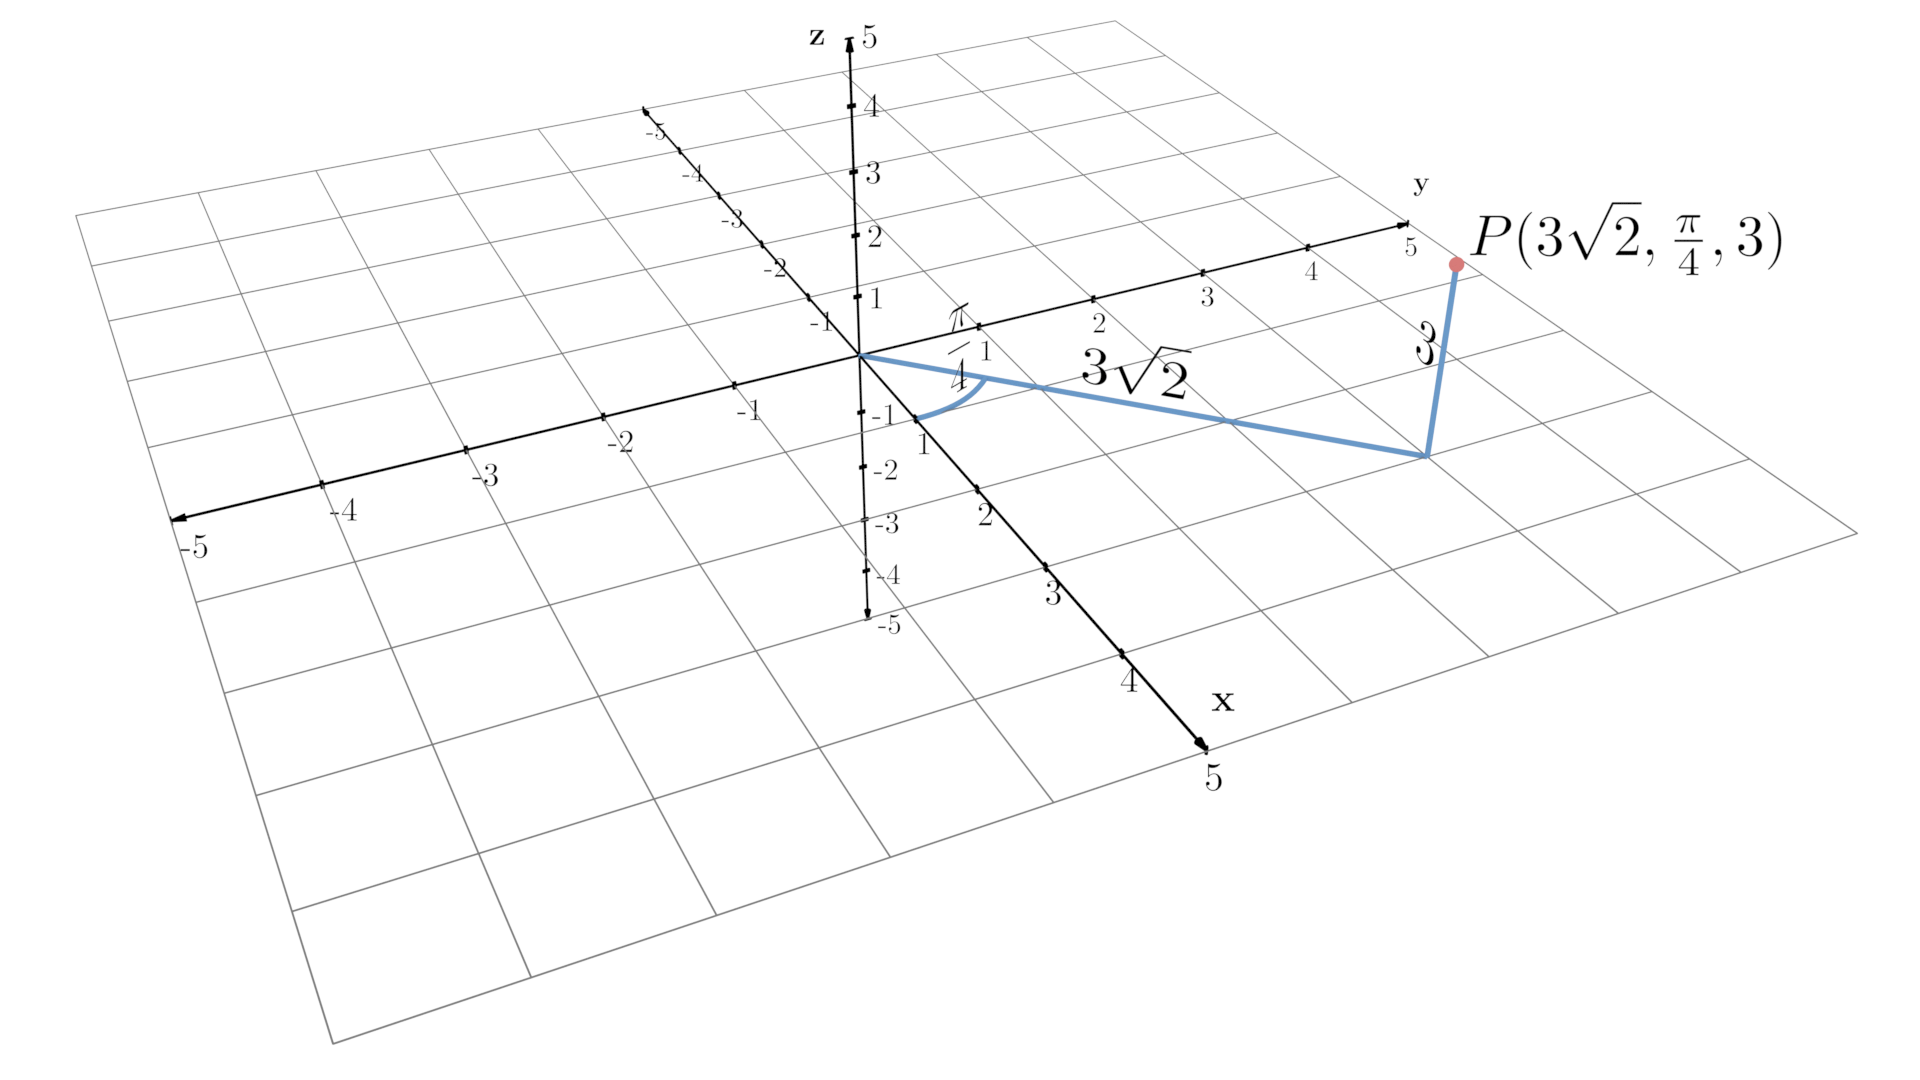
\includegraphics[width=0.711\linewidth]{Blender/cylindrical.png}
    \caption{3D cylindrical coordinate system.}
    \label{fig:cyli}
\end{figure}

According to Dawkins, there are alternate formulas for finding arc length that may be easier to use, especially when dealing with shapes that have some semblance of rotational symmetry \cite{Bib:polararc}. While this might be referred to as "polar coordinates" in two dimensions, three-dimensional space makes use of the cylindrical coordinate system$^[$\footnote{This defines a point using three numbers. The first number defines the shortest vector from the $z$-axis to the point. The second number defines the counterclockwise angle from the $x$-axis in which the radial vector points. The third number is the magnitude of the vertical vector. The point is at the sum of these two vectors.}$^]$ (Figure \ref{fig:cyli}) \cite{Bib:cylcords}.\par
First, gain a working understanding of the cylindrical coordinate system. Although it is not overly complicated, it may seem difficult at first glance. Next, determine the cylindrical parameterization for the general conical helix. This process will rely heavily on derivations from the previous section. Then, derive the 3D cylindrical arc length formula. The numerical method shown relies heavily on the 3D Cartesian arc length formula. Lastly, plug in the parameterization and evaluate.


\subsection{Derivation}\label{ssec:cyl}
\paragraph{THEOREM} The length of the helix spun $n$ times around the surface of a cone of base radius, $r$, and height, $h$, is $\sqrt{(\pi nr)^2+\frac{1}{4}\left(r^2+h^2\right)}-\frac{r^2+h^2}{4\pi nr}\ln\bigg|\frac{\sqrt{(2\pi nr)^2+r^2+h^2}-2\pi nr}{\sqrt{r^2+h^2}}\bigg|$ where $n,\ r,\ h>0$.
\smallskip
\paragraph{PROOF} Begin by deriving a parameterization in $r$, $\theta$, and $z$ of the conical helix both defined by the theorem above and of the type shown in Figure \ref{fig:helixlab}. Thanks to the previously derived equations \ref{eqns:helixcn} and the conversions supplied by Paul Dawkins \cite{Bib:cylcords}, this process will be straightforward. For reference, the following are a copy of equations \ref{eqns:helixcn}.
\begin{align*}
    x(t) &= (r-rt)\cos(2\pi nt)\\
    y(t) &= (r-rt)\sin(2\pi nt)\\
    z(t) &= ht
\end{align*}\par
The first important thing to know about cylindrical coordinates is that it still requires a parameter, $t$, i.e. $r$ and $z$ are not defined in terms of $\theta$. Because of this revelation, interval \ref{eqn:int} will still be needed in this section.\par
Let's begin writing the parameterization. Thanks to the previous work that culminated in equation \ref{eqn:rt}, one-third of the parameterization is already complete. Furthermore, Dawkins reveals in \cite{Bib:cylcords} that "$z=z$," so the last line of equations \ref{eqns:helixcn} can be used, making the parameterization two-thirds complete. Since $\theta$ must vary linearly from $0$ (its initial value) to $2\pi n$ (its maximum value) as $t$ varies from $0$ to $1$, $\theta(t)$ can be found using the slope formula, as follows. Note that a constant could be added to both starting and ending points of $\theta(t)$ similar to $t$ without affecting the calculus, but for simplicity's sake, this constant is likewise defined as zero.
\begin{align*}
    \theta(t) &= \frac{\Delta\theta}{\Delta t}t\\
    &= \frac{2\pi n-0}{1-0}t\\
    &= 2\pi nt
\end{align*}
Assemble the pieces to yield the final, cylindrical parameterization of the conical helix (equations \ref{eqns:helixcncyl}).
\begin{align}\label{eqns:helixcncyl}
    \begin{split}
        r(t) &= r-rt\\
        \theta(t) &= 2\pi nt\\
        z(t) &= ht
    \end{split}
\end{align}\par
Notably, this parameterization contains all of the same relevant information as equations \ref{eqns:helixcn} without any of the fluff of the sinusoidal functions.\par
Now that the parameterization has been obtained, the length of the defined helix can be found. However, the general three-dimensional arc length formula for cylindrical coordinates will be derived first. This process will be carried out in a manner adapted from Paul Dawkins' method for deriving the two-dimensional polar arc length formula \cite{Bib:polararc}. This is not so much a visual-graphical process as a numerical transformation of equation \ref{eqn:arcparam}. Dawkins suggests substituting the Cartesian conversion of the general cylindrical coordinate equations into the 2D arc length formula and simplifying. This will be carried out in 3D, as follows. Note that the Cartesian conversion is
\begin{align}\label{eqns:cartconv}
    \begin{split}
        x(t) &= r(t)\cos(\theta(t))\\
        y(t) &= r(t)\sin(\theta(t))\\
        z(t) &= z(t)
    \end{split}
\end{align}
Substitute equations \ref{eqns:cartconv} into equation \ref{eqn:arcparam} and simplify, as follows.
\begin{align*}
    \ell &= \int_a^b\sqrt{\left(\frac{d}{dt}(r(t)\cos(\theta(t)))\right)^2+\left(\frac{d}{dt}(r(t)\sin(\theta(t)))\right)^2+\left(\frac{dz}{dt}\right)^2}\, dt\\
    &= \int_a^b\sqrt{\left(\frac{dr}{dt}\cos(\theta(t))-r(t)\sin(\theta(t))\frac{d\theta}{dt}\right)^2+\left(\frac{dr}{dt}\sin(\theta(t))+r(t)\cos(\theta(t))\frac{d\theta}{dt}\right)^2+\left(\frac{dz}{dt}\right)^2}\, dt\tag{\theequation}\label{eqn:fin2}
    \stepcounter{equation}
\end{align*}
Pause to simplify the left two terms under the radical separately.
\begin{align*}
    &= \left(\frac{dr}{dt}\right)^2\cos^2(\theta(t))-2r(t)\sin(\theta(t))\cos(\theta(t))\left(\frac{dr}{dt}\right)\left(\frac{d\theta}{dt}\right)+r(t)^2\sin^2(\theta(t))\left(\frac{d\theta}{dt}\right)^2\\
    &\hspace{8em} +\left(\frac{dr}{dt}\right)^2\sin^2(\theta(t))+2r(t)\sin(\theta(t))\cos(\theta(t))\left(\frac{dr}{dt}\right)\left(\frac{d\theta}{dt}\right)+r(t)^2\cos^2(\theta(t))\left(\frac{d\theta}{dt}\right)^2\\
    &= \left(\frac{dr}{dt}\right)^2\cos^2(\theta(t))+\left(\frac{dr}{dt}\right)^2\sin^2(\theta(t))+r(t)^2\cos^2(\theta(t))\left(\frac{d\theta}{dt}\right)^2+r(t)^2\sin^2(\theta(t))\left(\frac{d\theta}{dt}\right)^2\\
    &= \left(\frac{dr}{dt}\right)^2\left(\cos^2(\theta(t))+\sin^2(\theta(t))\right)+r(t)^2\left(\frac{d\theta}{dt}\right)^2\left(\cos^2(\theta(t))+\sin^2(\theta(t))\right)\\
    &= \left(\frac{dr}{dt}\right)^2+r(t)^2\left(\frac{d\theta}{dt}\right)^2\tag{\theequation}\label{eqn:radical}
    \stepcounter{equation}
\end{align*}
Substitute equation \ref{eqn:radical} back into the corresponding part of equation \ref{eqn:fin2} to yield equation \ref{eqn:arcparam2}, the 3D arc length formula for an $r\theta z$-parameterized curve, such as equations \ref{eqns:helixcncyl}.
\begin{equation}\label{eqn:arcparam2}
    \ell = \int_a^b\sqrt{\left(\frac{dr}{dt}\right)^2+r(t)^2\left(\frac{d\theta}{dt}\right)^2+\left(\frac{dz}{dt}\right)^2}\, dt
\end{equation}
Plug equations \ref{eqns:helixcncyl} into equation \ref{eqn:arcparam2} and evaluate. Use the bounds given by interval \ref{eqn:int}.
\begin{align*}
    \ell &= \int_0^1\sqrt{\left(\frac{d}{dt}(r-rt)\right)^2+(r-rt)^2\left(\frac{d}{dt}(2\pi nt)\right)^2+\left(\frac{d}{dt}(ht)\right)^2}\, dt\\
    &= \int_0^1\sqrt{\left(-r\right)^2+(r-rt)^2(2\pi n)^2+h^2}\, dt\\
    &= \int_0^1\sqrt{(2\pi n)^2(r-rt)^2+r^2+h^2}\, dt\\
    &= \int_0^1\sqrt{(2\pi n(r-rt))^2+r^2+h^2}\, dt\tag{\theequation}\label{eqn:similar}
    \stepcounter{equation}
\end{align*}
In equation \ref{eqn:similar}, the cylindrical coordinate system has led back to equation \ref{eqn:later}.
\begin{flushright}
    \textbf{Q.E.D.}
\end{flushright}


\subsection{Summary}
With cylindrical coordinates, it is possible to define rotational shapes in three dimensions with fewer characters and functions. Such functions may require more setup before integrating to find the arc length, but are simpler to integrate, overall. I was first pointed to such a system by Dawkins \cite{Bib:cylcords}, who explained enough of the basics for me to adopt it for my own purposes. Although this method is not as different from the first as, say, the three methods in \cite{Bib:SORVolumes}, it does present a new and enlightening perspective.\par
There may be more methods (there is at least one more coordinate system: spherical coordinates), but this concludes those that will be explored in this paper.
\newpage



\setcounter{secnumdepth}{0}
\bibliography{ChristmasTree}
\bibliographystyle{ieeetr}
All figures are my own designs, created in Blender 3D with style influenced by Desmos. The sole exception is Figure \ref{fig:helixa}, which is my personal photograph.




\end{document}